\ifx\allfiles\undefined
\documentclass[12pt, a4paper, oneside, UTF8]{ctexbook}
\def\path{../config}
\usepackage{amsthm}
\usepackage{amssymb}
\usepackage{array}
\usepackage{xcolor}
\usepackage{graphicx}
\usepackage{mathrsfs}
\usepackage{enumitem}
\usepackage{geometry}
\usepackage[colorlinks, linkcolor=black]{hyperref}
\usepackage{stackengine}
\usepackage{yhmath}
\usepackage{extarrows}
\usepackage{tikz}
\usepackage{forest}
\usetikzlibrary{decorations.pathreplacing, positioning}
% \usepackage{unicode-math}
\usepackage{esint}
\usepackage{pifont}
\usepackage{tcolorbox}
\tcbuselibrary{skins, breakable}

\usepackage{multicol} 
\usepackage{fontspec} % 使用字体

\setmainfont{Times New Roman}
\setCJKmainfont{LXGWWenKai-Light}[
    SlantedFont=*
]

\usepackage{listings} % 用于插入代码

% 定义代码高亮风格
\lstset{
    basicstyle=\ttfamily\small,        % 基本字体样式(等宽小字体)
    keywordstyle=\color{blue},         % 关键字颜色
    commentstyle=\color{green},        % 注释颜色
    stringstyle=\color{red},           % 字符串颜色
    numbers=none,
    breaklines=true,                   % 自动换行
    frame=single,                      % 代码框边框
    rulecolor=\color{black},           % 边框颜色
    captionpos=b,                      % 标题位置(底部)
    showspaces=false,                  % 不显示空格标记
    showstringspaces=false,            % 不显示字符串中的空格标记
    language=C                         % 设置语言为 C
}

\usepackage{fontawesome5}

\usepackage{amsmath}
\usepackage{booktabs, array}
\usepackage{makecell}
\usepackage{fancyhdr}
\usepackage[dvipsnames, svgnames]{xcolor}
\usepackage{listings}
\usepackage{tasks}[2020/01/11]

\everymath{\displaystyle}

\definecolor{mygreen}{rgb}{0,0.6,0}
\definecolor{mygray}{rgb}{0.5,0.5,0.5}
\definecolor{mymauve}{rgb}{0.58,0,0.82}
\definecolor{NavyBlue}{RGB}{0,0,128}
\definecolor{Rhodamine}{RGB}{255,0,255}
\definecolor{PineGreen}{RGB}{0,128,0}

\graphicspath{ {figures/},{../figures/}, {config/}, {../config/} }

\linespread{1.6}

\geometry{
    top=25.4mm, 
    bottom=25.4mm, 
    left=20mm, 
    right=20mm, 
    headheight=2.17cm, 
    headsep=4mm, 
    footskip=12mm
}

\setenumerate[1]{itemsep=5pt,partopsep=0pt,parsep=\parskip,topsep=5pt}
\setitemize[1]{itemsep=5pt,partopsep=0pt,parsep=\parskip,topsep=5pt}
\setdescription{itemsep=5pt,partopsep=0pt,parsep=\parskip,topsep=5pt}



% \begin{lstlisting}[language=TeX] ... \end{lstlisting}

% 定理环境设置
% ---------- 颜色 ----------
\definecolor{ExBlue}{HTML}{4F81BD}
\definecolor{SolGreen}{HTML}{77933C}
\definecolor{DefRed}{HTML}{C5504B}
\definecolor{ThmOrange}{HTML}{E97132}
\definecolor{RemGray}{HTML}{7F7F7F}
\definecolor{CorPurple}{HTML}{7030A0}
\definecolor{ForGray}{HTML}{595959}

% ---------- 通用“变色”模板 ----------
\tcbset{
    mybox/.style n args={1}{
        enhanced, breakable,
        arc=6pt,
        boxrule=0.6pt,
        left=8pt, right=8pt, top=6pt, bottom=6pt,
        drop shadow={black!25},
        fonttitle=\bfseries,
        coltitle=white,
        colbacktitle=#1!85,
        colback=#1!10,
        colframe=#1,
    }
}

% ---------- 各环境 ----------
% 例题
\newtcolorbox{example}[1][]{mybox={ExBlue}, title={\ifstrempty{#1}{Example}{#1}}}
% 解答
\newtcolorbox{solution}[1][]{mybox={SolGreen}, title={\ifstrempty{#1}{Solution}{#1}}}
% 定义
\newtcolorbox{definition}[1][]{mybox={DefRed}, title={\ifstrempty{#1}{Definition}{#1}}}
% 定理
\newtcolorbox{theorem}[1][]{mybox={ThmOrange}, title={\ifstrempty{#1}{Theorem}{#1}}}
% 标注
\newtcolorbox{remark}[1][]{mybox={RemGray}, title={\ifstrempty{#1}{Remark}{#1}}}
% 推论
\newtcolorbox{corollary}[1][]{mybox={CorPurple}, title={\ifstrempty{#1}{Corollary}{#1}}}
% 公式
\newtcolorbox{formula}[1][]{mybox={ForGray}, title={\ifstrempty{#1}{Formula}{#1}}}


\settasks{
    label-format = \bfseries,
    label        = \Alph*.,
    label-width  = 1.2em,
    label-offset = 0.3em,
    item-indent  = 1.9em,
    column-sep   = 0.5em
}

\newenvironment{choices}[1][4]   % 默认 4 栏
    {\begin{tasks}(#1)}
    {\end{tasks}}

% 自定义命令的文件

\def\d{\mathrm{d}}
\def\R{\mathbb{R}}
\def\P{\partial} 
\newcommand{\bs}[1]{\begin{solution}#1\end{solution}}
\newcommand{\bt}[1][1]{% 默认参数为1
    \ensuremath{% 确保数学模式
        \foreach \n in {1,...,#1} {\blacktriangle}% 循环输出 #1 个黑色三角形
    }%
}

\newcommand{\bl}[1][1]{% 默认参数为1
    \ensuremath{% 确保数学模式
        \foreach \n in {1,...,#1} {\blacklozenge}% 循环输出 #1 个黑色三角形
    }%
}
\newif\ifshowanswers
%\showanswerstrue % 注释掉这行就不显示答案

% 定义答案环境
\newcommand{\answer}[1]{%
    \ifshowanswers
        #1%
    \fi
}




% 修改参数改变封面样式,0 默认原始封面、内置其他1、2、3种封面样式
\def\myIndex{3}


\ifnum\myIndex>0
    \input{\path/cover_package_\myIndex} 
\fi

\def\myTitle{冲刺150笔记}
\def\myAuthor{Weary Bird}
\def\myDateCover{\today}
\def\myDateForeword{\today}
\def\myForeword{行香子}
\def\myForewordText{
树绕村庄,水满陂塘;倚东风、豪兴徜徉。小园几许,收尽春光。有桃花红,李花白,菜花黄。 \\
远远苔墙,隐隐茅堂;飏青旗、流水桥旁。偶然乘兴,步过东冈。正莺儿啼,燕儿舞,蝶儿忙。 \\
}
\def\mySubheading{知错能改善莫大焉}


\definecolor{red}{HTML}{e74c3c}
\definecolor{black}{HTML}{2c3e50}
\begin{document}
% \input{../config/cover}
\else
\fi
\chapter{数据结构}
\section{选择题}
\begin{enumerate}
    \item \bt 下列程序段的时间复杂度是\_\_\_\_ 
    \begin{lstlisting}[language=C]
int sum = 0;
    for(int i = 1; i < n; i *= 2)
        for(int j = 0; j < i; j++)
            sum++;
    \end{lstlisting}

    \answer{
        \bs {
        假设第t次时$2^t\geq n$,此时$sum$执行的总次数为 
        $$
        1 + 2 + 4 + \ldots + 2^t = \frac{1-2^t}{1-2}=2^t - 1
        $$
        又因为$t=\log_2{n}$故而总的计算执行次数为$n-1\sim O(n)$
    }
    }

    \item 关于线性表的顺序存储和链式存储结构的描述中,正确的是(    ) 
    \begin{enumerate}
        \item [(1)] 线性表的顺序结构优于其链式存储结构
        \item [(2)] 链式存储结构比顺序存储结构能更方便地表示各种逻辑结构
        \item [(3)] 若频繁使用插入和删除操作,则顺序存储结构更优于链式存储结构
        \item [(4)] 顺序存储结构和链式存储结构都可以进行顺序存取 
    \end{enumerate}
    \begin{choices}
        \task 1,2,3
        \task 2,4
        \task 2,3
        \task 3,4
    \end{choices}
    \answer{
        \bs {
        选B 
        }
    }
    \item 对于一个头指针为$head$的带头结点的单链表,判断该表为空表的条件是(   ),对于不带头结点
    的单链表,判断空表的条件是(   ) 
    \begin{choices}[2]
        \task $head == NULL$ 
        \task $head\rightarrow next == NULL$ 
        \task $head\rightarrow next == head$ 
        \task $head \neq NULL$
    \end{choices}

    \answer{
        \bs{
            B,A 
        }
    }
    \item 一个链表最常用的操作为在末尾插入结点和删除节点,则选用(   )最节省时间. 
    \begin{choices}[2]
        \task 带头结点的双循环链表
        \task 单循环列表
        \task 带尾结点的单循环链表
        \task 单链表
    \end{choices}

    \answer{
        \bs {
            选A,可以注意分析时间复杂度.容易得到 \\
            对于A选项,分别为$O(1),O(1)$;对于B,C,D选项,分别为$O(n),O(n)$
        }
    }
    \item 设对$n(n>1)$元素的线性表运算只有4种,删除第一个元素,删除最后一个元素,在第一个元素之前插入
    一个元素,在最后一个元素之后插入一个元素,则最好使用(    ) 
    \begin{choices}[1]
        \task 只有尾结点指针没有头结点指针的循环单链表
        \task 只有尾结点指针没有头结点指针的非循环双链表
        \task 只有头结点指针没有尾结点指针的循环双链表
        \task 既有头结点有又有尾结点的循环单链表
    \end{choices}

    \answer{
        \bs {
            和上题一样逐一分析时间复杂度,选C.此时四种操作均可以达到$O(1)$的时间复杂度.
        }
    }
    \item 假定利用数组 $a[n]$ 存储一个栈,初始栈顶指针 $top==-1$,则元素x进栈的操作为() 
    \begin{choices}
        \task $a[--top] = x$ 
        \task $a[top--] = x$
        \task $a[++top] = x$
        \task $a[top++] = x$
    \end{choices}

    \answer{
        \bs {
            选C \\
            用数组模拟栈,具体的操作完全没比较记忆.毕竟$top=0$或者$top=-1$是完全不同的,掌握原理
            才是根本. \\
            考虑本题,由于$top=-1$,每次进栈前,应该先让$top+=1$在执行赋值操作,故应该为$top[++top]=x$;出栈操作为
            $top--$;
        }

        \begin{remark}[区分$++x$和$x++$]
            $++x$不会产生临时的副本,而是直接将$x+=1$的值返回给调用者; \\
            $x++$则会产生临时的$x$值,并将$x$的值返回给调用者后,将$x+=1$;
        \end{remark}
    }
    \item 和顺序栈相比,链栈有一个比较明显的优势,即() 
    \begin{choices}[2]
        \task 通常不会出现栈满的情况 
        \task 通常不会出现栈空的情况 
        \task 插入操作更容易实现 
        \task 删除操作更容易实现 
    \end{choices}

    \answer{
        \bs {
            选A \\
            顺序栈用数组实现,而数字的大小是指定的(不考虑动态申请数组空间的情况),而链栈用链表实现
            申请结点空间较为容易.故后者不容易出现栈满情况.
        }
    }
    \item 链栈(不带头结点)执行Pop操作,并将出栈元素存在x中,应该执行() 
    \begin{choices}[2]
        \task $x=top;top=top\rightarrow next$ 
        \task $x=top\rightarrow data$ 
        \task $top=top\rightarrow next;x=top\rightarrow data$
        \task $x=top\rightarrow data;top=top\rightarrow next$ 
    \end{choices}

    \answer{
        \bs {
            选D \\
            向将栈中的数据保存进$x$中,再将$top$指针后移(惰性删除,并不直接释放空间).
        }
    }
    \item 三个不同元素进栈,能够得到()不同的出栈序列 
    
    \answer{
        \bs {
            5个 \\
            对于n不大的情况,可以直接穷举.假设三个元素为$a,b,c$则穷举出栈序列即可 \\
            (1)$a,b,c$\qquad (2)$a,c,b$\qquad (3)$b,a,c$\\
            (4)$b,c,a$\qquad (5)$c,b,a$
        }

        \begin{remark}[求n个不同元素的出栈序列的个数]
            $$
            N=\frac{1}{n+1}C_{2n}^{n} 
            $$
            比如上题就可以用公式计算 
            $$
            \frac{1}{4}\cdot\frac{6*5*4}{3*2*1} = 5
            $$
        \end{remark}
    }
    \item 一个栈的输入序列为$1,2,\ldots,n$输出序列的第一个元素为i,则第j个输出元素是() 
    \begin{choices}
        \task 不确定
        \task n - i 
        \task n - i - 1
        \task n - i + 1
    \end{choices}

    \answer{
        \bs {
            选A,不确定
        }
    }

    \item 设栈的初始状态为空,当字符序列 \underline{n1\_}作为栈的输入时,输出长度为3,且可用做C语言
    标识符的序列有()个
    \begin{choices}
        \task 3
        \task 4
        \task 5
        \task 6
    \end{choices}
    \answer{
        \bs {
            答案选A,3个 \\
            C语言中变量标识符(变量名)只能以$\_$或者字母开头不能以数组开头.故只有3中可能的输出即\\
            $\_1n$ \qquad $n1\_$ \qquad $n\_ 1$
        }
    }
    \item 设有一个顺序共享栈Share[0:n-1],其中第一个栈顶指针top1的初始值为-1,第二个栈顶指针top2的初始值
    为n,则判断共享栈满的条件是() 
    \begin{choices}[2]
        \task $top2-top1\ ==\ 1$
        \task $top1-top2\ ==\ 1$ 
        \task $top1\ ==\ top2$ 
        \task 以上对不对
    \end{choices}

    \answer{
        \bs {
            选A \\
            第一个栈从$0\ldots,top1$;第二个栈从$top2,\ldots,n-1$只要两个栈指针相遇即$top1+1==top2$的时候
            共享栈就满了,此时$top2-top1==1$
        }
    }
    \item \bl 若元素\underline{a,b,c,d,e,f}依次进栈,允许进栈,出栈交替进行,但不允许连续3次进栈,退栈
    操作,不可能得到的出栈序列是() 
    \begin{choices}
        \task \underline{dcebfa}
        \task \underline{cbdaef}
        \task \underline{bcaefd}
        \task \underline{afedcb} 
    \end{choices}

    \answer{
        \bs {
            没有技巧,枚举的时候要考虑全面即可. 选D
        }
    }

    \item \bl 一个栈的入栈序列为\underline{$1,2,3\ldots,n$}出栈序列为$P_1,P_2,\ldots,P_n$.若$P_2=3$则$P_3$可能 
    的取值的个数是() 
    \begin{choices}
        \task n-3
        \task n-2
        \task n-1
        \task 无法确定 
    \end{choices}

    \answer{
        \bs {
            除$P_2=3$外其余全部数,即$n-1$选C
        }
    }
    \item \bl 若栈S1中保存整数,栈S2中保存运算符,函数F()依次执行如下各步操作: 
    \begin{enumerate}[label= (\arabic*)]
        \item 从S1中依次弹出两个操作数a和b
        \item 从S2中弹出一个运算符op
        \item 执行相应的运算b\ op\ a 
        \item 将运算结果压入S1中 
    \end{enumerate}
    假定S1中的操作数一次是\underline{5,8,3,2(2在栈顶)},S2中的运算符依次是\underline{*,-,+(栈顶)}.调用
    3次F()后,S1栈顶保存的值是() 
    \begin{choices}
        \task -15
        \task 15
        \task -20
        \task 20
    \end{choices}

    \answer{
        \bs {
            选B,模拟的时候注意题目要求$b\ op\ a$,$b$是第二次弹出的,$a$是第一次弹出的.
        }
    }
    \item 循环队列存储在数组$A[0\ldots n]$中,其中$rear$为队尾指针,$front$为队首指针.则入队时的操作为\_\_\_;
    出队时的操作为\_\_\_\_;判断队空的操作为\_\_\_;判断队满的操作为\_\_\_,当前队列中元素的个数为\_\_\_\_. 

    \answer{
        \bs {
            入队:$rear=(rear+1)\% (n+1); A[rear]=x$ \\
            出队:$front=(front+1)\%(n+1)$ \\
            判空:$rear=front$ \\
            判满:$(rear+1)\%(n+1)==front$
            当前队列中的元素: $(read-front+n+1)\%(n+1)$
        }
    }


    \item 用链式存储方法的队列进行删除操作时需要() 
    \begin{choices}[2]
        \task 仅修改头指针
        \task 仅修改尾指针
        \task 头尾指针都要修改
        \task 头尾指针可能都要修改 
    \end{choices}

    \answer{
        \bs {
            选D \\
            如果队列中元素不止一个,仅修改头指针;但如果队列中的元素仅一个的时候,就需要修改头指针和尾指针即$rear==front$
        }
    }

    \item 假设循环单链表表示的队列长度为n,队头固定在链表尾,若只设置头指针,则进队操作的时间复杂度为() 
    \begin{choices}
        \task $O(n) $ \task $O(1)$ \task $O(n^2)$ \task $O(n\log_{2}{n})$
    \end{choices}

    \answer{
        \bs {
            选A \\
            插入即在链头插入,此时时间复杂度是$O(1)$但为了保持循环单链表的性质,需要找到链尾(队头)元素,此时需要$O(n)$的时间复杂度.
        }
    }
    \item \bl 已知循环队列存储在一维数组$A[0\ldots n-1]$中,且队列非空时$front$和$rear$分别指向队头元素
    和队尾元素.若初始队列为空,且要求第一个进入队列的元素存储在$A[0]$处,则初始时$front$和$rear$的值分别是() 
    \begin{choices}
        \task 0,0 \task 0, n-1 \task n-1,0 \task n-1,n-1
    \end{choices}

    \answer{
        \bs {
            选B
        }
    }
    \item 循环队列放在一维数组$A[0\ldots M-1]$中, end1指向对首元素,end2指向队尾元素的后一个位置.假设
    队列两端均可进行入队与出队操作,队列中最多能容纳M-1个元素.初始时为空,下列判断队满和队空的条件中,正确的是() 
    \begin{choices}[1]
        \task 队空:$end1\ ==\ end2$ 队满: $end1\ ==\ (end2+1)\ mod\ M$ 
        \task 队空:$end1\ ==\ end2$ 队满: $end2\ ==\ (end1+1)\ mod\ (M-1)$
        \task 对空:$end2\ ==\ (end1+1)\ mod\ M$ 队满: $end1\ ==\ (end2+1)\ mod M$
        \task 对空:$end1\ ==\ (end2+1)\ mod\ M$ 队满: $end2\ ==\ (end1+1)\ mod (M-1)$
    \end{choices}

    \answer{
        \bs {
            选A
        }
    }
    \item \bl 已知操作符包含$+,-,*,/,(,)$.将中缀表达式$a+b-a*((c+d)/e-f)+g$转换为等价的后缀表达式(逆波兰表示法),
    用栈来实现.初始时栈为空,转换过程中栈中至多保存()个操作符. 

    \answer{
        \bs {
            5个 \\
            可以用栈直接做,也可以转化为二叉表达式树做(我感觉后者更好);当然前者也不能不会.
        }
    }

    \item \bt 有一个$n\times n$的对称矩阵$A$,将其下三角部分按行存放在一维数组B中,而$A[0][0]$存放在$B[0]$中,则
    第$i+1$行对角元素$A[i][i]$存放在B中的()处 
    \begin{choices}
        \task (i+3)i/2 
        \task (i+1)i/2
        \task (2n-i+1)i/2
        \task (2n-i-1)i/2 
    \end{choices}

    \answer{
        \bs {
            选A
        }
    }
    \item \bl 由一个100阶的三对角矩阵M,其元素$m_{i,j}(1\leq i, j\leq 100)$按行优先依次压入下标从0开始的一维
    数组N中.元素$m_{30,30}$在N中的下标是() 

    \answer{
        \bs {
            (1) 可以记公式$k=2i+j-3$ \\
            (2) 把三对角线矩阵画出来,观察. 第一个行元素为两个,在$m_{30,30}$所在行之前有$28$行这些行有3个元素;
            本行在$m_{30,30}$之前仅有$m_{30,29}$故$2+28\times+3+2 - 1 = 87$
        }
    }
    \item \bt 在KMP算法中,串\underline{ababaaababaa}的PM数组,Next数组,Nextval数组分别为? 
    \answer{
        \bs {
            (1) PM数组结果 \underline{001231123456} \\
            (2) Next(1)数组 \underline{-100123112345} \\
            (3) Next(2)数组 \underline{011234223456} \\
            (4) Nextval数组 \underline{010104210104}
        }
    }
    \item \bl 设主串$T=abaabaabcabaabc$模式串$S=abaabc$采用KMP算法进行模式匹配,到匹配成功为止,在匹配过程中进行的
    单个字符间的比较次数是()
    
    \answer{
        \bs {
            10次
        }
    }
    \item 树的路径长度是从树根到每个结点的路径长度的(   ) 
    \begin{choices}
        \task 总和
        \task 最小值
        \task 最大值
        \task 平均值
    \end{choices}

    \answer{
        \bs {
            树的路径长度:从树根到每个结点的路径长度的总和 \\
            树的带权路径长度(WPL):\\
            树中所有叶子结点的权值X该叶子到根的路径长度的总和 \\
            二者的区别在于,前者计算内部节点与叶子结点;而后者仅计算叶结点.
        }
    }
    \item (判断正误) 
    \begin{enumerate}
        \item [(1)] 度为2的有序树就是二叉树
        \item [(2)] 结点按完全二叉树层序编号的二叉树中,第$i$个结点的左孩子编号为$2i$ 
    \end{enumerate}
    
    \answer{
        \bs {
            错;\ 这二者的区别在于,对于二叉树,若一个结点仅有一个孩子,这个子结点是左孩子还是有孩子是
            确定的;而对于度为2的有序树,这个孩子是左孩子还是右孩子是无所谓的 \\
            错误;\ 左孩子不一定存在.
        }
    }

    \item 具有10个叶结点的二叉树中有(   )个度为2的结点 
    
    \answer{
        \bs {
            基本公式,对于二叉树有如下公式$n_0=n_2+1$;\\
            故$10-1=9$个度为2个结点
        }
    }
    \item 设二叉树有$2n$个结点,且$m<n$,则不可能存在(   )的结点 
    \begin{choices}
        \task n个度为0
        \task 2m个度为0
        \task 2m个度为1
        \task 2m个度为2
    \end{choices}

    \answer{
        \bs {
            选C \\
            由于$n_0=n_2-1$故一颗二叉树的总结点数目为$2n=n_1+2n_2+1$则$n_1=2(n-n_2)-1$显然
            $n_1$必须是奇数,必然不可能有$2m(\text{偶数})$个度为1的结点
        }
    }
    \item 已知一颗完全二叉树的第6层(设根为第一层)有8个结点,则完全二叉树的结点个数最少是(   ) 

    \answer{
        \bs {
            39 \\
            由于完全二叉树的特性可知,当高度为6的时候结点数目最小且前5层必然是满二叉树,故此时完全
            二叉树的结点个数最小是$2^5-1+8=39$个结点
        }
    }
    \item 一颗完全二叉树上有1001个结点,其中叶结点的个数是(    ) 

    \answer{
        \bs {
            501 \\
            解法一:\ 对于完全二叉树,若其结点数为n,则最后一个分支结点(含子结点)的序号为$x=\lfloor n/2 \rfloor$
            当$n_i>x$的时候说明该结点是叶子结点. 故本题,最后一个分支结点的序号为$\lfloor 1001/2 \rfloor=500$
            故叶结点的序号范围为$501\sim 1001$,总数为501 \\
            解法二:\ 由于$n=2n_0+n_1-1$由于完全二叉树的定义可知$n_1=0$或者$n_1=1$带入可以知$n_1=0,n_0=501$
        }
    }
    \item \bl 对于任意一颗高度为5且有10个结点的二叉树,若采用顺序存储结构保存,每个节点占1个存储单元(仅保存
    结点的数据信息),则存放该二叉树需要的存储单元数量至少是(     ) 

    \answer{
        \bs {
            31 \\
            这道题比较容易错,数字存储二叉树必须按照满二叉树存储,因为并不能事先知道那些叶结点会有; 
            故这道题的答案是$2^5-1=31$
        }
    }
    \item 在下列关于二叉树遍历的说法中,正确的是(     ) 
    \begin{choices}[1]
    \task 若有一个结点是二叉树中某个子树的中序遍历结果序列的最后一个结点,则它一定是该子树的前序遍历结果序列的最后一个结点。
    \task 若有一个结点是二叉树中某个子树的前序遍历结果序列的最后一个结点,则它一定是该子树的中序遍历结果序列的最后一个结点。
    \task 若有一个叶结点是二叉树中某个子树的中序遍历结果序列的最后一个结点,则它一定是该子树的前序遍历结果序列的最后一个结点。
    \task 若有一个叶结点是二叉树中某个子树的前序遍历结果序列的最后一个结点,则它一定是该子树的中序遍历结果序列的最后一个结点。
    \end{choices} 

    \answer{
        \bs {
            选C,这种题举反例即可,注意题设.
        }
    }
    \item 设$n,m$为一颗二叉树上的两个结点,在后序遍历时,$n$在$m$前的充分条件是(    ) 
    \begin{choices}
        \task n在m的右方 
        \task n是m的祖先
        \task n在m的左方
        \task n是m的子孙 
    \end{choices}

    \answer{
        \bs {
            选D \\
            C选项要加上二者位于同一层,才是充分条件. 
        }
    }
    \item 在二叉树中的两个结点m和n,若m是n的祖先,则使用(    )可以找到从m到n的路径 
    
    \answer{
        \bs {
            后序遍历 \\
            在遍历过程中,从根(或子树根m出发)后序遍历会先走完m的整棵子树才回溯,因此可以在访问到n时沿着递归栈或显式栈回溯,
            从而得到 m→…→n 的路径
        }
    }
    \item 若二叉树中结点的先序序列是$\ldots a\ldots b\ldots$,中序序列是$\ldots b\ldots a\ldots$则(    ) 
    \begin{choices}[1]
        \task 结点a和结点b分别在某结点的左子树和右子树中
        \task 结点b和结点a的右孩子中
        \task 结点b在结点a的左孩子中
        \task 结点a和结点b分别在某结点的两颗分非空子树中 
    \end{choices}

    \answer{
        \bs {
            选C 
        }
    }
    \item 线索二叉树是(    )结构 
    \begin{choices}
        \task 逻辑
        \task 逻辑和存储
        \task 物理
        \task 线性
    \end{choices}

    \answer{
        \bs {
            选C \\
            逻辑结构=“是什么关系”——只关心数据之间的逻辑关系(线性、树、图等),与机器怎么存、存在哪儿无关。 \\
            物理结构=“怎么存”——关心在内存/磁盘里到底怎么摆放(顺序表、链表、索引、散列、线索化等实现细节)。 \\
            二叉树本身是一种逻辑结构,而线索二叉树是加上前后指针后的链式结构.
        }
    }
    \item 一颗左子树为空的二叉树的先序线索化后,其中空的链域的个数是(    ) 
    \begin{choices}
        \task 不确定
        \task 0个
        \task 1个
        \task 2个
    \end{choices} 

    \answer{
        \bs {
            选D 
        }
    }
    \item 二叉树在线索化后,仍然不能有效求解的问题是(    ) 
    \begin{choices}[2]
        \task 先序线索二叉树求先序后继
        \task 中序线索二叉树求中序后继
        \task 中序线索二叉树求中序前驱
        \task 后序线索二叉树求后序后继 
    \end{choices}

    \answer{
        \bs {选D}
    }
    \item 若X是二叉中序线索树中一个有左孩子的结点,且X不为根,则X的前缀为(    ) 
    \begin{choices}[2]
        \task X的双亲
        \task X的右子树中最左节点
        \task X的左子树中最右结点
        \task X的左子树中最右的叶结点
    \end{choices}

    \answer{
        \bs {选C}
    }

    \item (   )遍历仍然需要栈的支持. 
    \begin{choices}
        \task 先序线索树
        \task 中序线索树
        \task 后序线索树 
        \task 所有线索树 
    \end{choices}

    \answer{
        \bs {
            选C \\
            后序线索树中,根的后序后继是父结点,但普通线索二叉树没有保存父指针;
            当右子树非空时,无法通过线索直接得到该后继,仍需借助栈来回溯。
        }
    }
    \item \bl 先序序列为\underline{a,b,c,d}的不同二叉树的个数是(      ) 

    \answer{
        \bs {
            14 \\
            简单来说等价于求4个元素的卡特兰数,即
            $$
            n = \frac{1}{n+1}C_{2n}^{n} = 14
            $$ 
            任何一棵n个结点的二叉树,其先序遍历序列与中序遍历序列的对应关系等价于n个元素的入栈顺序与出栈顺序的对应关系; \\
            先序遍历与入栈顺序一致 \\
            中序遍历与出栈顺序一致 \\
            故上述问题转换为入栈顺序为\underline{a,b,c,d},则出栈序列的个数是啥?
        }
    }
    \item \bl 若结点p和q在二叉树T的中序遍历序列中相邻,且p在q之前,则下列p和q的关系中,不可能的是(    )
    \begin{enumerate}
        \item [(1)] q是p的双亲 
        \item [(2)] q是p的右孩子
        \item [(3)] q是p的右兄弟
        \item [(4)] q是p的双亲的双亲
    \end{enumerate}
    \begin{choices}
        \task 1 
        \task 3
        \task 2,3
        \task 2,4
    \end{choices}

    \answer{
        \bs {选B} 
    }

    \item 利用二叉链表存储森林时,根结点的右指针是(    ) 
    \begin{choices}
        \task 指向最左兄弟 
        \task 指向最右兄弟 
        \task 一定为空
        \task 不一定为空 
    \end{choices}

    \answer{
        \bs {
        选D  \\
        森林与二叉树的转换依据(左孩子右兄弟表示法)若森林内只有一颗树,则右指针为空;但若不止一棵树
        则右指针非空. 
        }
    }
    \item 森林$T=(T_1,T_2,\ldots,T_m)$转换为二叉树BT的过程为:若m=0,则BT为空,若$m\neq 0$,则(    ) 
    \begin{choices}[1]
        \task 将中间子树$T_{mid}(mid=(1+m)/2)$的根作为BT的根;将$(T_1,T_2,\ldots,T_{mid-1})$转换为BT的左子树;
        将$(T_{mid+1},\ldots,T_m)$转换为BT的右子树 
        \task 将子树$T_1$的根作为BT的根,将$T_1$的子树森林转换为BT的左子树;将$(T_2,T_3\ldots,T_m)$转换BT的右子树 
        \task 将子树$T_1$根作为BT的根,将$T_1$的左子森林转换为BT的左子树;右子森林转换右子树,其他类似 
        \task 将森林T的根作为BT的根,将$(T_1,\ldots,T_m)$转换为该根下的结点,得到一棵树,然后将这课树转换为二叉树 
    \end{choices}


    \answer{
        \bs {
            选B \\
            将森林的每棵树视为兄弟结点,再按照左孩子右兄弟的规则来转换.
        }
    }
    \item 设F是一个森林,B是由F转换为来的二叉树.若F中有n个非终端节点,则B中右指针域为空的结点数目是(    ) 

    \answer{
        \bs {
            n+1 \\
            二叉树B中右指针为空的结点表明该结点无无兄弟结点. \\
            其中森林中所有根结点中仅最右边的根的右指针为空,所有中间结点的孩子中,必然有且仅有一个孩子右指针为空(n个) \\
            综上有$n+1$个右指针为空
        }
    }
    \item \bl 将森林转换为对应的二叉树,若二叉树中,结点u是结点v的父结点的父结点,则原来的森林中,u和v可能具有关系是(   ) 
    \begin{enumerate}
        \item [(1)] 父子关系 
        \item [(2)] 兄弟关系
        \item [(3)] u的父结点和v的父结点是兄弟关系
    \end{enumerate}
    \begin{choices}
        \task 2 
        \task 1,2
        \task 1,3
        \task 1,2,3 
    \end{choices}

    \answer{
        \bs {
            选B \\
            这个III,老头想问的是 "在原来森林中u的父结点和v的父结点"是不是兄弟,而不是问转换后的二叉树
            "u的父结点和v的父结点"在原来的森林中是不是兄弟关系.
        }
    }
    \item \bl 已知一颗有2011个结点的树,其叶结点个数为116,则该树对应的二叉树中无右孩子的结点个数为(   )
    \begin{choices}
        \task 115
        \task 116
        \task 1895
        \task 1896
    \end{choices}

    \answer{
        \bs {
            1896 \\
            这道题和46题考察的内容一致. 每个分支结点的最右孩子必然无右指针,根结点也必然无(单棵树),故$n-n_0+1=1896$
        }
    }
    \item \bl 若森林F有15条边,25个结点,则F包含树的个数是(    ) 

    \answer{
        \bs {
            10 \\
            对于一棵树其结点与边数满足(n=e-1),对于每棵树其节点数比边数多1,而本题结点比边数多$25-15=10$棵树.
        }
    }
    \item \bl 若将一颗树T转换为对应的二叉树BT,则下列对BT的遍历中,其遍历序列与T的后根遍历序列相同的是(   ) 
    \begin{choices}
        \task 先序遍历
        \task 中序遍历
        \task 后序遍历
        \task 层序遍历
    \end{choices}

    \answer{
        \bs {
            选B \\
            对于一颗多叉树与二叉树的转换后的遍历关系有如下: \\
            先根遍历(多叉树) $\rightarrow$ 先序遍历(二叉树) \\
            后根遍历(多叉树) $\rightarrow$ 中序遍历(二叉树) \\
            多叉树没有所谓的中根遍历. 
        }
    }
    \item 在有n个叶节点的哈夫曼树中,非叶结点的总数是(   ) 
    
    \answer{
        \bs {
            $n-1$ \\
            (二叉)哈夫曼树的重要特征:仅包含度为0或者度为2的节点.又因为非空二叉树满足$n_2=n_0-1$故非叶结点
            总数为$n-1$
        }
    }
    \item 设哈夫曼编码的长度不超过4,若已对两个字符编码为1和01,则还最多可以对(   )个个字符编码 
    
    \answer{
        \bs {
            4 \\
            哈夫曼编码是前缀编码,3位编码可以是(000)此时四位编码可以是(0010,0011);同理3为编码是(001)时候,四位
            编码为(0010,0011)是不是答案就是3呢?并不是,并没有说一定要有3位编码,若只用4为编码此时可能的编码有(0000,0001,0010,0011)
            有4种编码方式. 
        }
    }
    \item 一下对于哈夫曼树的说法中,错误的是(    ) 
    \begin{choices}[1]
        \task 对应一组权值构造出来的哈夫曼树一般不是唯一的
        \task 哈夫曼树具有最小的带权路径长度
        \task 哈夫曼树中没有度为1的结点
        \task 哈夫曼树中除了度为1的节点外,还有度为2的结点和叶结点 
    \end{choices}

    \answer{
        \bs {
            选D \\
            考虑哈夫曼树的构造过程,每次选取和最小的两个结点作为叶结点.而这两个结点何者为左
            结点,何者为右结点是不确定,故哈夫曼树通常是不唯一的. 
        }
    }
    \item 若度为m的哈夫曼树中,叶结点的数目为n,则非叶结点的数目为(     ) 
    
    \answer{
        \bs {
            $\lceil(n-1)/(m-1)\rceil$ \\
            由于哈夫曼树的特性可知,m叉哈夫曼树仅有度为0和度为m的结点.设总结点数为$N=n_0+n_m$又因为
            N个结点的哈夫曼树有$N-1$条分支,则$mn_m=N-1=n_m+n_0-1$即$n_m=(n_-1)/(m-1)$
        }
    }
    \item \bl 已知字符集\underline{a,b,c,d,e,f}若各字符出现的次数分别为\underline{6,3,8,2,10,4}则对应字符集中的
    各字符的哈夫曼编码可能是(    ) 
    \begin{choices}[2]
        \task \underline{00,1011,01,1010,11,100} 
        \task \underline{00,100,110,000,0010,01}
        \task \underline{10,1011,11,0011,00,010}
        \task \underline{0011,10,11,0010,01,000}
    \end{choices}

    \answer{
        \bs {
            选A \\
            注意构建哈夫曼树,至于左右孩子谁为0谁为1是不确定.可以带入选项判断. 
        }
    }
    \item \bl 对应任意给定的含有n个字符的有限集合S,用二叉树表示S的哈夫曼编码集和定长编码集,分别得到二叉树$T_1$和$T_2$.下列叙述
    正确的是(    ) 
    \begin{choices}[1]
        \task $T_1$和$T_2$的结点数相同
        \task $T_1$的高度大于$T_2$的高度
        \task 出现频次不同的字符在$T_1$中处于不同的层
        \task 出现频次不同的字符在$T_2$中处于相同的层
    \end{choices}

    \answer{
        \bs {
            选D 
        }
    }

    \item 以下关于图的叙述中,正确的是(    ) 
    \begin{choices}[1]
        \task 图与树的区别在于图的边数大于等于顶点数 
        \task 假设有图$G=\{V,\{E\}\}$,顶点集$V'\subseteq V, E' \subseteq E$则$V'$和$\{E'\}$构成$G$的子图 
        \task 无向图的连通分量是指无向图的极大连通子图 
        \task 图的遍历就是从图中的某一顶点出发遍历图中的其余顶点 
    \end{choices}

    \answer{
        \bs {
            选C \\
            树无环且连通,边数恰好是n-1;而图没有这种限制. \\
            B选项第一眼很容易理解错,子图还要求$E'$中每一条边对应的结点都存在于$V'$中,否则不是合法图. \\
            对于非连通图,通过一个结点并不能一次遍历其余所有结点 
        }
    }

    \item 以下关于图的说法,正确的是(   ) 
    \begin{choices}[1]
        \task 强连通有向图的任何顶点到其他顶点都有弧 
        \task 图的任意顶点的入度都等于出度 
        \task 有向完全图一定是强连通有向图 
        \task 有向图的边集的子集和顶点集的子集可构成原有向图的子图 
    \end{choices}

    \answer{
        \bs {
            选C \\
            A: 强连通(连通)图仅保证结点和结点之间有\textbf{路径}而不保证有弧(边) \\
            B: 只有无向图的入度等于出度,而有向图并不一定满足 \\
            D: 如上题C一致. 
        }
    }
    \item 对于一个有$n$个顶点的图;若是连通无向图,其边的个数至少是(   );若是强连通有向图,其边的个数至少为(   ) 
    
    \answer{
        \bs {
            $n-1;n$ \\
            最小的连通无向图即一颗树,此时边为(n-1);而对于有向图,构成一个有向环,此时边为(n);
        }
    }
    \item 在有$n$个顶点的有向图中,顶点的度最大可以达到(    ) 
    
    \answer{
        \bs {
            $2n-2$ \\
            由于408数据结构仅考虑简单图,每个结点最多只能与其余$n-1$个结点存在两条互相指向的弧,即每个顶点
            出度=入度=$n-1$,综上顶点的度之和为$2n-2$ 
        }
    }

    \item 设无向图$G=(V,E),G'=(V',E')$若$G'$是$G$的生成树,则下列不正确的是(   ) 
    \begin{enumerate}
        \item [(1)] $G'$为$G$的连通分量 
        \item [(2)] $G'$为$G$的无环子图
        \item [(3)] $G'$为$G$的极小连通子图且$V'=V$   
    \end{enumerate}
    \begin{choices}
        \task 1,2 \task 3 \task 2,3 \task 1
    \end{choices}

    \answer{
        \bs {
            选D
        }
    }
    \item \bl 下列关于无向连通图特性的叙述中,正确的是(  ) 
    \begin{enumerate}
        \item [(1)] 所有顶点的度之和为偶数 
        \item [(2)] 边数大于顶点数减一 
        \item [(3)] 至少有一个顶点的度为一 
    \end{enumerate}
    \begin{choices}
        \task 1 \task 2 \task 1,2 \task 1,3 
    \end{choices}

    \answer{
        \bs {
            选A \\
            对于无向图$I$总是成立,考虑一棵树其边数等于顶点数减一但此时是连通的,所以$II$错误;考虑成环的无向图,此时每个
            点的度都为2的倍数,故$III$错误. 
        }
    }

    \item 带权有向图G用临接矩阵存储,则$v_i$的入度等于邻接矩阵中(    )
    \begin{choices}[2]
        \task 第i行非$\infty$的元素个数
        \task 第i列非$\infty$的元素个数
        \task 第i行非$\infty$且非0的元素个数
        \task 第i列非$\infty$且非0的元素个数
    \end{choices}

    \answer{
        \bs {
            选D \\
            这道题讲道理有歧义,除非默认$0$表示无边否则应该选B. 
        }
    }

    \item 无向图G中包含N(N>15)个顶点,以临接矩阵形式存储时共占用$N^2$个存储单元(其他辅助空间忽略不计);以临接表
    形式存储时,每个表结点占用3个存储单元,每个头结点占用2个存储单元(其他辅助空间忽略不计).若令图$G$的临接矩阵存储所占空间
    小于等于临接表存储所占空间,该图$G$所包含的边的数量至少是(   ) \\

    \answer{
        \bs {
            $(N^2-2N)/6$ \\
            不要忘记无向图表要存两次 
        }
    }

    \item n个顶点的无向图的邻接表中最多有(   )个边表节点
    
    \answer{
        \bs {
            $n(n-1)$ \\
            临接表有两部分,一部分为顶点表(存顶点)一部分为边表(存边);从而当其是一个完全图的时候边数最多
            此时有$n(n-1)$条边,从而边表结点有$n(n-1)$个 
        }
    }
    \item 假设有n个顶点,e条边的有向图用邻接表表示,则删除与某个顶点v相关的所有边的
    时间复杂度是(    ) 

    \answer{
        \bs {
            $O(n+e)$ \\
            分类加,分步乘,这里是分类;  \\
            删除顶点$v$的出边,直接顺着顶点表,删除这个顶点即可.$O(n)$ \\
            删除顶点$v$的入边,遍历整张临接表的所有顶点,并把以含$v$的边表结点删除,此时每边至多遍历一次$O(e)$ \\
            综上,最终的时间复杂度为$O(n+e)$
        }
    }

    \item 对于一个有n个顶点,e条边的图采用临接表表示时,进行DFS遍历的时间复杂度是(   ),空间复杂度是
    (   );进行BFS遍历的时间复杂度是(   ),空间复杂度是(    ) 

    \answer{
        \bs {
            $O(n+e),O(n);O(n+e),O(n)$ \\
            空间复杂度不包含临接表的开销, DFS主要是递归栈的消耗,由于要遍历每个点一次最多需要压入$n$个点;BFS
            使用队列实现,最多同时有$n$个顶点入队. 
        }
    }
    \item 对于一个有n个顶点,e条边的图采用临接矩阵表示时,进行DFS遍历的时间复杂度是(   ),空间复杂度是
    (   );进行BFS遍历的时间复杂度是(   ),空间复杂度是(    ) 

    \answer{
        \bs {
            $O(n^2),O(n);O(n^2),O(n)$ \\
            注意这里的空间复杂度不包含临接矩阵的消耗;此时消耗和上题没有区别; 
        }
    }
    \item 图的广度优先生成树的树高比深度优先生成的树高(    ) 
    \begin{choices}
        \task 小或相等
        \task 小 
        \task 大或相等 
        \task 大
    \end{choices}

    \answer{
        \bs {
            小或相等 
        }
    }

    \item 从无向图的任意顶点出发进行一次深度优先遍历便可以访问所有顶点,则该图一定是(   ) \\
    \begin{choices}
        \task 完全图 
        \task 连通图 
        \task 有回路 
        \task 一棵树 
    \end{choices}

    \answer{
        \bs {
            选B \\
            一棵树可以通过一次DFS遍历所有点,但并非所有连通图都是一棵树.  
        }
    }

    \item 一下叙述中,正确的是(   ) 
    \begin{choices}[1]
        \task 最短路径一定是简单路径
        \task Dijkstra算法不适合求有环路的带权图的最短路径
        \task Dijkstra算法不适合求任意两个顶点的最短路径 
        \task Floyd算法求两个顶点的最短路径,$path_k-1$一定是$path_k$的子集 
    \end{choices}

    \answer{
        \bs {
            选A \\
            若环的权值之和为负数,此时通过反复过环路径长度为无穷小,不存在所谓最短路;若环权值为0,此时
            完全不需要经过这个环可以直接删除;若环权值之和为正数$w>0$,设环形路径为$P=s\rightarrow
            \ldots\rightarrow u\rightarrow C\rightarrow u\ldots\rightarrow t$ 其中C是一个环路,
            把C删除得到新的路径为$P'=s\rightarrow\ldots\rightarrow u\rightarrow u\ldots\rightarrow t$
            显然$W(P')=W(P)-W(C)<W(P)$因此最短路必然不包含正权回路.  \\
            $Dijkstra$算法能够处理\textbf{不含负权环路}的最短路径而非不含环路,对于零(正)权回路的最短路问题一样可以做 \\
            $Dijkstra$每次可以确定两个顶点间的最短路,只要每个顶点都使用一次就可以确定任意顶点间的最短路 \\
            Floyd维持的最优子结构是距离值的递推,即
            $$
            d_{ij}^{k} = \min\{d_{ij}^{k-1},d_{ik}^{k-1}+d_{kj}^{k-1}\}
            $$
            而非维护路径集合. Floyd算法更新规则为若$d_{ik}^{k-1}+d_{kj}^{k-1}<d_{ij}^{k=1}$直接把从$i$到$j$的新路径设置为
            $$
            path[i][j]=path[i][k]+path[k][j] 
            $$
            整段可能被完全抛弃所以不符合路径子集.
        }
    }
    \item 若一个有向图的顶点不能排成一个拓扑序列,则可以判断该有向图(    ) 
    \begin{choices}[2]
        \task 含有多个出度为0的顶点
        \task 是一个强连通图
        \task 含有多个入度为0的顶点
        \task 含有顶点数大于1的强连通分量 
    \end{choices}

    \answer{
        \bs {
            选D \\
            拓扑排序存在$\iff$ 有向图无环 
        }
    }
    \item 下列关于图的说法中,正确的是(   ) 
    \begin{enumerate}
        \item [(1)] 有向图中顶点V的度等于其临接矩阵中第V行中1的个数
        \item [(2)] 无向图的邻接矩阵一定是对称矩阵,有向图的邻接矩阵一定是非对称矩阵
        \item [(3)] 在带权图$G$的最小生成树$G_i$中,某条边的权值可能会超过为选边的权值
        \item [(4)] 若有向无环图的拓扑序列唯一,则可以唯一确定该图 
    \end{enumerate}
    \begin{choices}
        \task 1,2,3
        \task 3,4
        \task 3
        \task 4
    \end{choices}

    \answer{
        \bs {
            选C \\
            I: 有向图应该考虑行与列, $\text{度}=\text{入度}+\text{出度}=\sum_{j=1}^{n}A[j][i]+\sum_{j=1}^{n}A[i][j]$  \\
            II: 有向图只要入度等于出度,其临接矩阵也是对称矩阵 \\
            III: 最小生成树只能保证其权值之和为所有生成树中权值最少,但边权最少的边并不一定能组成一个生成树 \\
            IV: 考虑如下两图,其拓扑排序一致但图不一致. 
            \begin{center}
                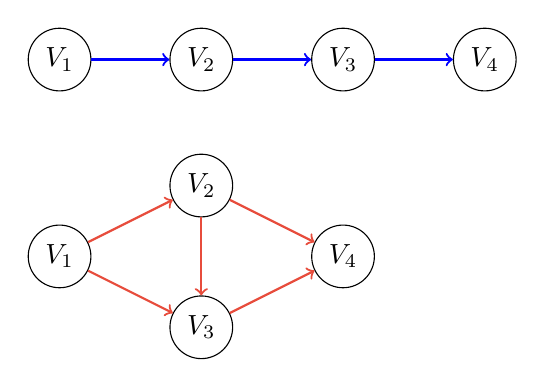
\begin{tikzpicture}[node distance=1.8cm,
                        every node/.style={circle,draw,minimum size=6mm}]
                %----------------  图 1  ----------------
                \node (v1) at (0,0)  {$V_1$};
                \node (v2) at (1.8,0) {$V_2$};
                \node (v3) at (3.6,0) {$V_3$};
                \node (v4) at (5.4,0) {$V_4$};
                \path[->,thick,blue]
                (v1) edge (v2)
                (v2) edge (v3)
                (v3) edge (v4);

                %----------------  图 2  ----------------
                \begin{scope}[yshift=-2.5cm]
                \node (u1) at (0,0)  {$V_1$};
                \node (u2) at (1.8,0.9) {$V_2$};
                \node (u3) at (1.8,-0.9) {$V_3$};
                \node (u4) at (3.6,0) {$V_4$};
                \path[->,thick,red]
                (u1) edge (u2)
                (u1) edge (u3)
                (u2) edge (u3)
                (u2) edge (u4)
                (u3) edge (u4);
                \end{scope}

                \end{tikzpicture}
            \end{center}
        }
    }
    \item 已知带权图为$G=(V,E)$,其中$V=\{v_1,v_2,\ldots,v_{10}\}$,边集合为$E=\{<v_1,v_2>5,
    <v_1,v_3>6,<v_2,v_5>3,<v_3,v_5>6,<v_3,v_4>3,<v_4,v_5>3,<v_4,v_7>1,<v_4,v_8>4,<v_5,v_6>4,
    <v_5,v_7>2,<v_6,v_{10}>4,<v_7,v_9>5,<v_8,v_9>2,<v_9,v_{10}>2\}$则G的关键路径长度为(   ) 

    \answer{
        \bs{
            21
        }
    }

    \item 下列关于关键路径的说法中,正确的是(   ) 
    \begin{enumerate}
        \item [(1)]改变网上某一关键路径上的某一关键路径,必将产生不同的关键路径
        \item [(2)]在AOE图中,关键路径上活动的时间延长多少,整个工期的时间也就随之延长多少
        \item [(3)]缩短关键路径上任意一个关键活动的持续时间可缩短关键路径长度
        \item [(4)]缩短所有关键路径上共有的任意一个关键活动的持续时间可缩短关键路径的长度
        \item [(5)]缩短多条关键路径上共有的任意一个关键活动的持续时间可缩短关键路径长度 
    \end{enumerate}
    \begin{choices}
        \task 2,5
        \task 1,2,4
        \task 2,4
        \task 1,4
    \end{choices}

    \answer{
        \bs {
            选C 
        }
    }
    \item \bl 若用临接矩阵存储有向图,矩阵中主对角线以下的元素全为零,则关于该图拓扑序列的结论是(   )
    \begin{choices}[2]
        \task 存在,且唯一
        \task 存在,且不唯一
        \task 存在,可能唯一
        \task 无法确定是否存在
    \end{choices}

    \answer{
        \bs {
            选C \\
            题设条件只能保证有向图无环,而不能保证拓扑排序唯一.当前仅当每次确定拓扑序时只能找到一个入度为0的点,此时
            拓扑排序唯一.  \\
            在离散数学中确实有拓扑序列唯一的充要条件\textbf{G的Hasse图是一条链}
        }
    }
    \item \bl 对下列图所示的有向带权图,若采用Dijkstra算法求源点a到其他个顶点的最短路径,则得到的
    的第一条最短路径的目标顶点是b,第二条最短路径的目标顶点是c,后续得到的其余各最短路径的目标顶点一次是(   )
    \begin{center}
        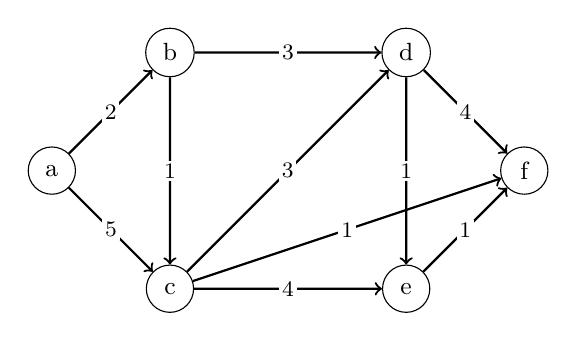
\begin{tikzpicture}[scale=1.5,
        vertex/.style={circle, draw, minimum size=6mm, font=\small},
        edge/.style={->, thick},
        label/.style={font=\footnotesize, pos=.5, auto=center, fill=white, inner sep=1pt}
    ]

    % 顶点
    \node[vertex] (a) at (-2,-2) {a};
    \node[vertex] (b) at (-1,-1) {b};
    \node[vertex] (c) at (-1,-3) {c};
    \node[vertex] (d) at (1,-1) {d};
    \node[vertex] (e) at (1,-3) {e};
    \node[vertex] (f) at (2,-2) {f};

    % 有向边
    \draw[edge] (a) -- node[label] {2} (b);
    \draw[edge] (a) -- node[label] {5} (c);
    \draw[edge] (b) -- node[label] {1} (c);
    \draw[edge] (b) -- node[label] {3} (d);
    \draw[edge] (c) -- node[label] {3} (d);
    \draw[edge] (c) -- node[label] {1} (f);
    \draw[edge] (c) -- node[label] {4} (e);
    \draw[edge] (d) -- node[label] {1} (e);
    \draw[edge] (d) -- node[label] {4} (f);
    \draw[edge] (e) -- node[label] {1} (f);

    \end{tikzpicture}
    \end{center}
    \begin{choices}
        \task d,e,f 
        \task e,d,f 
        \task f,d,e 
        \task f,e,d
    \end{choices}


    \answer{
        \bs {
            选C \\
            需要熟练理解下面的过程,很重要! 
            \begin{center}
            \begin{tabular}{c|c|c|c|c|c}
                \hline
                顶点 & 第一轮 & 第二轮 & 第三轮 & 第四轮 & 第五轮 \\
                \hline 
                b & $\color{red}(a,b)2$ & - & - & - & - \\
                \hline
                c & $(a,c)5$ & $\color{red}(a,b,c)3$ & - & - & - \\
                \hline 
                d & $\infty$ & $(a,b,d)5$ & $(a,b,d) 5$ & $\color{red} (a,b,d) 5$ & - \\
                \hline
                e & $\infty$ & $\infty$ & $(a,b,c,e) 7$ & $(a,b,c,e)7$ & $\color{red} (a,b,d,e)6$ \\
                \hline
                f & $\infty$ & $\infty$ & $\color{red} (a,b,c,f)4$ & - & - \\
                \hline 
                集合S & $(a,b)$ & $(a,b,c)$ & $(a,b,c,f)$ & $(a,b,c,f,d)$ & $(a,b,c,f,d,e)$ \\
                \hline
            \end{tabular}
            \end{center}
        }
    }
    \item \bl 使用Dijkstra算法求下图中从顶点1到其他个顶点的最短路径,依次得到的各最短路径的目标
    顶点是(   )

    \begin{center}
    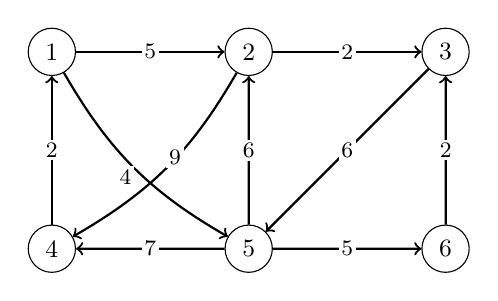
\begin{tikzpicture}[scale=2.5,
    vertex/.style={circle, draw, minimum size=6mm, font=\small},
    edge/.style={->, thick},
    label/.style={font=\footnotesize, pos=.5, auto=center, fill=white, inner sep=1pt}
    ]

    % 顶点
    \node[vertex] (1) at (0,0) {1};
    \node[vertex] (2) at (1,0) {2};
    \node[vertex] (3) at (2,0) {3};
    \node[vertex] (4) at (0,-1) {4};
    \node[vertex] (5) at (1,-1) {5};
    \node[vertex] (6) at (2,-1) {6};

    % 有向边(1→5 用弧线下弯,2→4 用弧线上弯)
    \draw[edge,bend right=15] (1) to node[label,below left=-1pt] {4} (5);
    \draw[edge,bend left =15] (2) to node[label,above right=-1pt] {9} (4);

    % 其余直线边
    \draw[edge] (1) -- node[label] {5} (2);
    \draw[edge] (2) -- node[label] {2} (3);
    \draw[edge] (3) -- node[label] {6} (5);
    \draw[edge] (4) -- node[label] {2} (1);
    \draw[edge] (5) -- node[label] {6} (2);
    \draw[edge] (5) -- node[label] {7} (4);
    \draw[edge] (5) -- node[label] {5} (6);
    \draw[edge] (6) -- node[label] {2} (3);

    \end{tikzpicture}
    \end{center}

    \begin{choices}
        \task 5,2,3,4,6
        \task 5,2,3,6,4
        \task 5,2,4,3,6
        \task 5,2,6,3,4
    \end{choices}

    \answer{
        \bs {
            5,2,6,3,4 \\
            和上题一样,思考上图的那个表即可. 
        }
    }
    \item \bl 下列所示的AOE网表示一项包含8个活动的工程,活动d的最早开始时间和最迟开始时间分别是(   ) 

    \begin{center}
    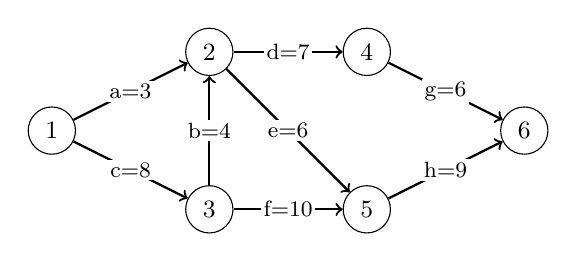
\begin{tikzpicture}[scale=2,
    vertex/.style={circle, draw, minimum size=6mm, font=\small},
    edge/.style={->, thick},
    label/.style={font=\footnotesize, pos=.5, auto=center, fill=white, inner sep=1pt}
    ]

    % 顶点
    \node[vertex] (1) at (0,0) {1};
    \node[vertex] (2) at (1,0.5) {2};
    \node[vertex] (3) at (1,-0.5) {3};
    \node[vertex] (4) at (2,0.5) {4};
    \node[vertex] (5) at (2,-0.5) {5};
    \node[vertex] (6) at (3,0) {6};

    \draw[edge] (1) -- node[label] {a=3} (2);
    \draw[edge] (1) -- node[label] {c=8} (3);
    \draw[edge] (2) -- node[label] {d=7} (4);
    \draw[edge] (2) -- node[label] {e=6} (5);
    \draw[edge] (3) -- node[label] {b=4} (2);
    \draw[edge] (3) -- node[label] {f=10} (5);
    \draw[edge] (4) -- node[label] {g=6} (6);
    \draw[edge] (5) -- node[label] {h=9} (6);
    \end{tikzpicture}
    \end{center}
    \begin{choices}
        \task 3,7
        \task 12,12
        \task 12,14
        \task 15,15
    \end{choices}

    \answer{
        \bs {
            12和14
        }
        \begin{definition}[AOE网络的计算过程] 
            具体参看笔记,这里只给出上题的计算过程的表格.\\
            时间的最早开始时间(拓扑)前驱结点的最早开始时间+对应活动之和的\text{最大值} \\
            时间的最迟开始时间(拓扑)后继结点的最迟开始时间-对应活动之差的\text{最小值} 
            \begin{center}
            \begin{tabular}{p{3.5cm}|p{4.5cm}|p{4.5cm}}
                \hline
                事件(按拓扑序) & 最早开始时间 & 最迟开始时间  \\ 
                \hline
                1(源点)& 0 & 0 \\
                \hline 
                3 & 0 + 8 = 8 & $\min\{12-4,18-10\}=8$  \\
                \hline
                2 & $\max\{3,8+4\}$ = 12 & $\min\{19-7,18-6\}=12$ \\
                \hline
                5 & 12+6=18 & 27-9=18 \\
                \hline
                4 & 12+7=19 & 27-6=21 \\
                \hline
                6(汇点) & $\max\{19+6,18+9\}=27$ & 27(关键路径长度) \\
                \hline
            \end{tabular}
            \end{center}
            事件的最早开始时间该事件(弧)对应的弧尾所表示时间的最早开始时间 \\
            事件的最迟开始时间该事件(弧)对应弧头所示的最迟开始时间与该活动持续时间之间 
            \begin{center}
            \begin{tabular}{p{3.5cm}|p{4.5cm}|p{4.5cm}}
                \hline
                活动 & 最早开始时间 & 最迟开始时间  \\ 
                \hline
                a & $EST[1]=0$ & $LST[2]-3=9$ \\
                \hline 
                b & $EST[3]=8$ & $LST[2]-4=8$  \\
                \hline
                c & $EST[1]=0$ & $LST[3]-8=0$ \\
                \hline
                d & $EST[2]=12$ & $LST[4]-7=14$ \\
                \hline
                e & $EST[2]=12$ & $LST[5]-6=12$ \\
                \hline
                f & $EST[3]=8$ & $LST[5]-10=8$ \\
                \hline
                g & $EST[4]=19$ & $LST[6]-6=21$ \\
                \hline 
                h & $EST[5]=18$ & $LST[6]-9=18$ \\
                \hline
            \end{tabular}
            \end{center}
        \end{definition}
    }

    \item 图G利用十字链表法表示如下,请问图$G$可能的拓扑排序为(    ) 
    \begin{center}
    \includegraphics[scale=0.35]{十字链表.png}
    \end{center}
    \begin{choices}
        \task $V_2,V_0,V_3,V_1,V_4$ 
        \task $V_0,V_3,V_1,V_4,V_2$ 
        \task $V_2,V_0,V_4,V_3,V_1$ 
        \task 不存在拓扑序列
    \end{choices}

    \answer{
        \bs {
        选C \\
        这道题的关键在于如何通过十字链表复原这个图.十字链表的解读参考笔记. 
        复原后的图如下 
        \begin{center}
        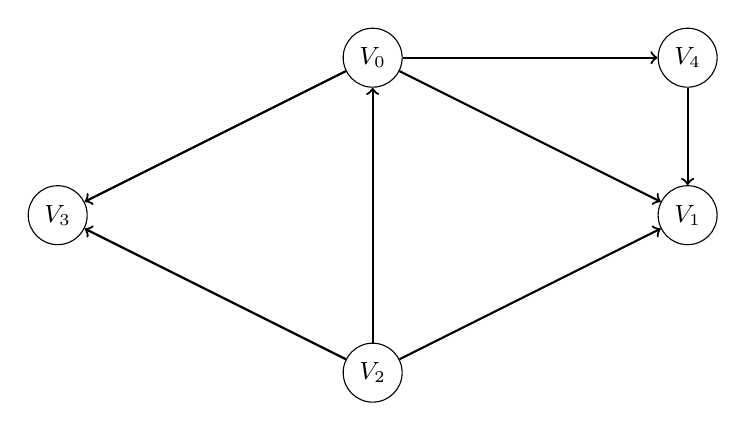
\begin{tikzpicture}[scale=2,
        vertex/.style={circle, draw, minimum size=6mm, font=\small},
        edge/.style={->, thick},
        ]

        % 顶点
        \node[vertex] (0) at (1,1) {$V_0$};
        \node[vertex] (1) at (3,0) {$V_1$};
        \node[vertex] (2) at (1,-1) {$V_2$};
        \node[vertex] (3) at (-1,0) {$V_3$};
        \node[vertex] (4) at (3,1) {$V_4$};

        \draw[edge] (0) -- node {} (1);
        \draw[edge] (0) -- node {} (3);
        \draw[edge] (0) -- node {} (4);
        \draw[edge] (2) -- node {} (0);
        \draw[edge] (2) -- node {} (3);
        \draw[edge] (2) -- node {} (1);
        \draw[edge] (4) -- node {} (1);

        \end{tikzpicture}
        \end{center}
        }
    }

    \item 以下对于最小生成树的描述,正确的是(   ) 
    \begin{enumerate}
        \item [(1)] 所有无向连通图的最小生成树一定有多个 
        \item [(2)] $Prim$和$Kruskal$算法构建的最小生成树一定不同 
        \item [(3)] 只要无向图中不存在相同权值的边,则该无向图的最小生成树唯一 
        \item [(4)] 只要无向图中存在权值相同的边,则该无向图的最小生成树一定不唯一
        \item [(5)] 在具有n个顶点的无向图G中,含有n个顶点,n-1条边的G的子图就是G的生成树 
        \item [(6)] 生成树就是最小生成树 
    \end{enumerate}
    \begin{choices}
        \task 3 \task 3,4 \task 全部正确 \task 全部错误 
    \end{choices}

    \item 以下说法中错误的是(   ) 
    \begin{enumerate}
        \item [(1)] 求从源点到其余顶点的Dijkstra最短路径算法中弧上权不能为负的原因是在实际应用中无意义 
        \item [(2)] 若图用临接矩阵表示,则利用Dijkstra算法求每一对不同顶点之间的最短路径的算法时间为$O(n^3)$ 
        \item [(3)] Floyd算法求每对不同顶点对的算法中允许弧上的权为负,但不能有权和为负的回路 
    \end{enumerate}
    \begin{choices}
        \task 1,2,3 \task 1 \task 1,3 \task 2,3 
    \end{choices}

    \item ()可以求无向图的所有连通分量.  

    \answer{
        \bs {
            $dfs,bfs$ 
        }
    }
    \item 存在一张无向连通图$G=(V,E),\left|V\right|=n,\left|E\right|=e$分布使用$Prim,Kruskal$算法来产生图
    G的最小生成树,则时间复杂度分别是(  ). 

    \answer{
        \bs {
            $O(n^2),O(e\log_{2}{e})$
        }
    }

    \item 已知7个城市(分别编号$0\sim 6$)之间修建道路的耗费分别为: \\
    (0,1)22,(0,2)9,(0,3)10,(1,3)15,(1,4)15,(1,6)12,(2,3)4,(2,5)3,(3,5)5,(3,6)23,(4,6)20,(5,6)32\\
    要修建路网让每两个城市间都可以互通(直达或途径其他城市),最小的耗费是(    ); 

    \answer{
        \bs {
            50 
        }
    }

    \item 由n个数据元素组成的两个表:一个递增有序,一个无序.采用顺序查找算法,对有序表从头开始查找,发现当前
    元素已不小于待查元素时,停止查找,确定查找不成功,已知查找任意元素的概率是相同的,则在两种表中成功查找(   ) 
    \begin{choices}[2]
        \task 平均时间后者小
        \task 平均时间两者相同
        \task 平均时间前者小
        \task 无法确定
    \end{choices}

    \answer{
        \bs {
            选B \\
            对于顺序查找,不管线性表是有序的,成功查找第一个元素的比较次数都是1,成功查找的第二个元素比较次数都是2,
            依次类推,每个元素查找成功的比较次数只和位置有关而与线性表是否有序无关.
        }
    }
    \item 在一个顺序存储的有序线性表上查找一个数据时,既可以采用折半查找,也可以采用顺序查找,但前者
    比后者的查找速度(   ) 
    \begin{choices}[2]
        \task 必然快
        \task 取决于表是递增还是递减
        \task 在大部分情况下要快
        \task 必然不快 
    \end{choices}

    \answer{
        \bs {
            选C 
        }
    }
    \item 折半查找过程所对应的判断树是一颗(   ) 
    \begin{choices}
        \task 最小生成树
        \task 平衡二叉树
        \task 完全二叉树
        \task 满二叉树
    \end{choices}

    \answer{
        \bs {
            选B 
        }
    }
    \item 折半查找和二叉排序树的时间性能(   ) 
    \begin{choices}
        \task 相同
        \task 有时不相同
        \task 完全不同
        \task 无法比较
    \end{choices}

    \answer{
        \bs {
            选B 
        }
    }
    \item 对表长为n的有序表进行折半查找,其判定树的高度为(    ) 
    \begin{choices}
        \task $\lceil\log_{2}{(n+1)}\rceil$
        \task $\log_{2}{(n+1)}-1$
        \task $\lceil\log_{2}{n}\rceil$
        \task $\lfloor\log_2{n}\rfloor$ - 1
    \end{choices}
    
    \answer{
        \bs {
            选A 
        }
    }
    \item 具有12个关键字的有序表中,对每个关键的查找概率相同,折半查找算法查找成功的平均查找长度是(   ),
    折半查找失败的平均查找长度是(    ) 

    \answer{
        \bs {
            $\frac{37}{12},\frac{49}{12}$ \\
            这种题比较理想的做法是画出该关键字序列的判定树,用虚拟失败结点和叶结点计算失败与成功查找长度.不妨假设
            含12个关键字的有序表为$0,1,\ldots,11$此时其折半查找判定树为. 
            \begin{center}
            \begin{forest}
            for tree={
            circle, draw, minimum size=6mm,
            inner sep=1pt, font=\small,
            s sep=6mm
            }
            [5
            [2
                [0[x][1[x][x]]]
                [3[x][4[x][x]]]
            ]
            [8
                [6[x][7[x][x]]]
                [10[9[x][x]][11[x][x]]]
            ]
            ]
            \end{forest}
            \end{center}
            查找成功的
            $$
            ASL=(1+2x2+3x4+4x5)/12 = \frac{37}{12}
            $$
            查找失败的 
            $$
            ASL=(3x3+4x10)/12 = \frac{49}{12}
            $$
            注意查找失败计算的时候不要多加虚拟的失败节点! 
        }   
    }
    \item 为提高查找效率,对有65025个元素的有序顺序表建立索引顺序结构,在最好的情况下查找到表中已有元素最多
    需要执行(   )次关键字比较 
    
    \answer{
        \bs {
            16 \\
            为了使查找效率最高,每个索引块的大小应该是$\sqrt{n}=\sqrt{65025}=255$,此时索引项的个数为$\frac{65025}{255}=255$,若
            此时采用折半查找,效率最高,$2x\log_{2}(255+1)=16$
        }
    }
    \item \bl 已知一个长度为16的顺序表L,其元素按关键字有序排列,若采用折半查找法查找一个L中不存在的元素,则
    关键字的比较次数最多是(    ) 

    \answer{
        \bs {
            查找失败最多只需要查找整个树高即$\lceil \log_{2}(n+1) \rceil$
        }
    }

    \item \bl 下列二叉树中,可能成为折半查找判定树(不含外部结点)的是
    \begin{center}
    \includegraphics[scale=0.35]{17-折半查找.png}
    \end{center}

    \answer{
        \bs {
            选A \\
            这道题第一眼可以以为是考察折半查找的判定树必然是一棵平衡树,然后发现所有选项都是平衡树.
            然后想呀想,二分还有啥特性呢?其决策树必然是一棵排序树,但好像没啥用.还有啥特性呢? \\
            其实谜底在谜面上,二分最重要的当然是确定分界点呀,因此不妨根据中序有序把数字全部还原回去看看分界点的
            确定是否满足二分的要求. 
        }
    }
    
    \item 在含有n个结点的二叉排序中查找某个关键字的结点时,最多进行(   )比较 
    \answer{
        \bs {
            n \\
            二叉排序树最差会退化为单链表. 
        }
    }
    \item 构建一颗具有n个节点的二叉排序树时,最理想情况下的深度为(   )
    \answer{
        \bs {
            $\lceil \log_2{n+1} \rceil$
        }
    }
    \item 含有20个节点的平衡二叉树的最大深度为(   ),具有5层结点的AVL树至少有(   )个结点.
    \answer{
        \bs {
            6,12 \\
            关键在于AVL结点树的递推公式,$n_0=0,n_1=1,n_{h}=n_{h-1}+n_{h-2}$
        }
    }


    \item 下列关于红黑树的说法中,正确的是(   ) 
    \begin{choices}[1]
        \task 红黑树的红结点的数目最多和黑结点的数目相同
        \task 若红黑树的所有结点都是黑色的,那么它一定是一棵满二叉树
        \task 红黑树的任何一个分支结点都有两个非空孩子结点
        \task 红黑树的子树也一定是红黑树
    \end{choices}

    \answer{
        \bs {
            选B \\
            对于B选项,红黑树的重要特征之一是黑平衡,所以当一个红黑树全为黑结点必然是满二叉树,否则就会破坏黑平衡条件 \\
            对于D选项,由于红黑树要求根为黑结点,所有根节点为红色的都不是红黑树. 
        }
    }
    \item \bt 将关键字序列\underline{1,2,3,4,5,6,7}一次插入初始为空的红黑树T,则T中红结点的个数是(    ) 
    \answer{
        \bs {
            3个 \\
            红黑树的插入过程比较重要(考察可能性比删除高,删除太难了.) 
        \forestset{
            rbt/.style={
                for tree={circle, draw, minimum size=6mm, font=\small,
                        inner sep=1pt, s sep=3mm, l sep=6mm},
                red/.style={fill=red!80, text=white},
                black/.style={fill=black!80, text=white}
            }
        }
        \begin{center}
        \begin{forest}rbt
            [1,black]
        \end{forest}\quad
        \begin{forest}rbt
            [1,black[,black][2,red]]
        \end{forest}\quad 
        \begin{forest}rbt
            [2,black[1,red][3,red]]
        \end{forest}\quad
        \begin{forest}rbt
            [2,black[1,black][3,black[,black][4,red]]]
        \end{forest}
        \begin{forest}rbt
            [2,black[1,black][4,black[3,red][5,red]]] 
        \end{forest}
        \begin{forest}rbt
            [2,black[1,black][4,red[3,black][5,black[,black][6,red]]]]
        \end{forest}
        \begin{forest}rbt
            [2,black[1,black][4,red[3,black][6,black[5,red][7,red]]]]
        \end{forest}
        \end{center}
    }
}
    \item \bl 现有一颗无重复关键字的平衡二叉树,对其进行中序遍历得到一个降序序列,下列关于该平衡二叉树的叙述中,正确的是(  ) 
    \begin{choices}[2]
        \task 根结点的度一定是2
        \task 树中最小元素一定是叶结点
        \task 最后插入的元素一定是叶结点
        \task 树中最大元素一定是无左子树
    \end{choices}

    \answer{
        \bs {
            选D\\
            根据题设有左子树>根>右子树. 最小元素只能保证无右子树而不能保证是叶子结点.最大元素可以保证无左子树. 
        }
    }
    \item \bl 在任意一颗非空平衡二叉树$T_1$中,删除某结点v之后形成平衡二叉树$T_2$,再将v插入$T_2$形成
    平衡二叉树$T_3$下列关于$T_1,T_3$的描述中,正确的是(   )
    \begin{enumerate}
        \item [(1)] 若v是$T_1$的叶结点,则$T_1$和$T_3$可能不相同 
        \item [(2)] 若v不是$T_1$的叶结点,则$T_1$和$T_3$一定不相同
        \item [(3)] 若v不是$T_1$的叶节点,则$T_1$和$T_3$一定相同 
    \end{enumerate}
    \begin{choices}
        \task 1
        \task 2
        \task 1,2
        \task 1,3
    \end{choices}
    \answer{
        \bs {
            选A 
        }
    }
    \item 下列关于B与B+树的描述中,不正确的是(   ) 
    \begin{choices}[2]
        \task B数和B+树都能有效的支持顺序查找
        \task B树和B+树都能有效的支持随机查找
        \task B树和B+树都是平衡的多叉树
        \task B树和B+树都可以用于文件索引结构
    \end{choices}

    \answer{
        \bs {
            选A \\
            仅带链的B+树支持顺序查找
        }
    }
    \item \bl 已知一颗3阶B树,如下图所示.删除关键字78得到一颗新B树,其最右叶结点中的关键字是(   )
    \begin{center}
        \begin{forest}
        for tree={rectangle,draw,minimum size=6mm,inner sep=2pt,edge=-}
        [45[17 35 [10][21][37]][55 65[47][60 62][78]]]
        \end{forest}
    \end{center}

    \answer{
        \bs {
            65 \\
            对于3阶B树,其关键字范围为$\lceil 3/2 \rceil \sim 3 -1 = 1 \sim 2$ \\
            其左兄弟的关键字为$2\geq\lceil3/2\rceil$属于够接的情况,删除后的B树如下
        \begin{center}
            \begin{forest}
            for tree={rectangle,draw,minimum size=6mm,inner sep=2pt,edge=-}
            [45[17 35 [10][21][37]][55 62[47][60][65]]]
            \end{forest}
        \end{center}
        }
    }
    \item \bl 在一颗高度为2的5阶B树中,所含有的关键的个数至少是(   ) 
    \begin{choices}
        \task 5
        \task 7
        \task 8
        \task 14
    \end{choices}

    \answer{
        \bs {
            选A \\
            B树的根结点至少有两个子结点(包含一个关键字),其余分支结点的关键字范围为$\lceil 5/2\rceil - 1 \sim 5 - 1 = 2\sim 4$,所以
            包含关键字最少的情况如下,个数为(1+2+2)
            \begin{center}
                \begin{forest}
                for tree={rectangle,draw,minimum size=6mm,inner sep=2pt,edge=-}
                [x[x x[][][]][x x[][][]]]
                \end{forest}
            \end{center}
        }
    }
    \item \bl 下列应用中,适合使用B+树的是(   ) 
    \begin{choices}[2]
        \task 编译器中的词法分析
        \task 关系数据库系统的索引
        \task 网络中的路由表的快速查找
        \task 操作系统的磁盘空闲块管理
    \end{choices}

    \answer{
        \bs {
            选B 
        }
    }

    \item 散列表查找成功时,平均查找长度仅和()有关. 
    \answer{
        \bs {
            填充因子
        }
    }
    \item 在开放定址法中散列到同一地址而引起的堆积问题是由于(   )而引起的
    \begin{choices}[2]
        \task 同义词之间发生冲突
        \task 非同义词之间发生冲突
        \task 同义词之间或非同义词之间发生冲突 
        \task 散列表溢出 
    \end{choices}

    \answer{
        \bs {
            选C 
        }
    }

    \item 下列关于散列冲突处理方法中,正确的是(   ) 
    \begin{enumerate}
        \item [(1)] 采用在平方探测法处理冲突时不容易产生聚集
        \item [(2)] 采用线性探测法解决冲突时,所有同义词在散列表中一定相邻
        \item [(3)] 采用链地址法处理冲突时,若限定在链首插入,则插入任意一个元素的时间是相同的 
        \item [(4)] 采用链地址法处理冲突时容易引起聚集现象
    \end{enumerate}

    \begin{choices}
        \task 1,3 \task 1,2,3 \task 3,4 \task 1,4
    \end{choices}

    \answer{
        \bs {
            选A 
        }
    }
    \item 对包含n个元素的散列表进行查找,平均查找长度为(   ) 
    \begin{choices}
        \task 为$O(\log_{2}{n})$
        \task 为$O(1)$
        \task 不直接依赖于n
        \task 直接依赖于表长m
    \end{choices}

    \answer{
        \bs {
            选C \\
            仅和填充因子有关 
        }
    }

    \item \bl 现有长度为11且初始为空的散列表HT,散列函数$H(k)=k\%7$,用线性探测再散列法法解决冲突,将
    关键字序列\underline{87,40,30,6,11,22,98,20}依次插入HT后,HT查找失败的平均查找长度是(   )
    \begin{choices}
        \task 4
        \task 5.25
        \task 6
        \task 6.29
    \end{choices}
    
    \answer{
        \bs {
            选C \\
            哈希表的查找成功和查找失败的平均查找长度是重点,需要掌握.  \\
            查找成功计算关键字的比较次数,查找失败计算"插槽".  \\
            最后哈希表如下所示 
            \begin{center}
            \begin{tabular}{c|c|c|c|c|c|c|c|c|c|c|c|c}
                \hline 
                散列地址 & 0 & 1 & 2 & 3 & 4 & 5 & 6 & 7 & 8 & 9 & 10 & 11 \\
                \hline 
                关键字 & 98 & 22 & 30 & 87 & 11 & 40 & 6 & 20 &  &  &  \\
                \hline 
            \end{tabular}
            \end{center}
            对于算出关键字算出的地址为0,需要比较$0\sim 8$地址的关键字才能确定失败;对于关键字算出地址为1,
            需要比较$1\sim 8$,一次类推;需要注意原关键字序列算不出$7$,哈希表中的20是被线性探测改到的位置,所以只有7个位置是可能的. 
            $$
            ASL_{fail}=\sum_{i=0}^{6}\frac{9-i}{7} = 6
            $$
        }
    }
    \item \bl 下列因素中,影响哈希方法的平均查找长度是(   ) 
    \begin{enumerate}
        \item [(1)] 装填因子
        \item [(2)] 散列函数
        \item [(3)] 冲突解决策略
    \end{enumerate}
    \begin{choices}
        \task 1,2
        \task 1,3
        \task 2,3
        \task 1,2,3
    \end{choices}

    \answer{\bs{选D}} 

    \item 下列关于排序的叙述中,正确的是(   ) 
    \begin{choices}[1]
        \task 稳定的排序方法优于不稳定的排序方法
        \task 对同一线性表使用不同的排序方法进行排序,得到的排序结果可能不同
        \task 排序方法都是在顺序表上实现的,在链表上无法实现排序方法
        \task 在顺序表上实现的排序方法在链表上也可以实现
    \end{choices}

    \answer{
        \bs {
            选B \\
            注意并非所有排序方法都可以用于链表,例如折半插入排序(用于要使用二分)链表就无法实现. 但大部分应该还是可以的. 
        }
    }

    \item 对于任意7个关键字进行基于比较的排序,至少要进行()次关键字之间的比较
    \begin{choices}
        \task 13
        \task 14
        \task 15
        \task 16
    \end{choices}

    \answer{
        \bs {
            选A \\
            对于任意n个关键字排序的比较次数,其下界为$\lceil\log_{2}(n!)\rceil$ 
        }
    }
    \item 用直接插入排序算法对下列4个表进行排序(从小到大),比较次数最少的是(   ) 
    \begin{choices}[2]
        \task \underline{94,32,40,90,80,46,21,69}
        \task \underline{21,32,46,40,80,69,90,94}
        \task \underline{32,40,21,46,69,94,90,80}
        \task \underline{90,69,80,46,21,32,94,40}
    \end{choices}

    \answer{
        \bs {
            选B \\
            插入排序中,越解决正序插入次数越少.
        }
    }
    \item 对序列\underline{98,36,-9,0,47,23,1,8,10,7}采用希尔排序,下列序列( )是增量为4的一趟排序结果 
    \begin{choices}[2]
        \task \underline{10,7,-9,0,47,23,1,8,98,36}
        \task \underline{-9,0,36,98,1,8,23,47,7,10}
        \task \underline{36,98,-9,0,23,47,1,8,7,10}
        \task 以上都不对
    \end{choices}

    \answer{
        \bs {
            选A 
        }
    }
    \item 若用冒泡排序算法对序列\underline{10,14,26,29,41,52}从大到小进行排序,则需要进行(  )比较 
    \begin{choices}
        \task 3
        \task 10
        \task 15
        \task 25
    \end{choices}

    \answer{
        \bs {
        选C
        }
    }


    \item 对下列关键字序列用到了快排进行排序,速度最快的情形是()速度最慢的是() 
    \begin{choices}[2]
        \task \underline{21,25,5,17,9,23,30}
        \task \underline{25,23,30,17,21,5,9}
        \task \underline{21,9,17,30,25,23,5}
        \task \underline{5,9,17,21,23,25,30}
    \end{choices}

    \answer{
        \bs {A,D}
    }
    \item 对于下列4个序列,以第一个关键字为基准用快速排序算法进行排序,在第一趟过程中移动记录次数最多的是()
    \begin{choices}[2]
        \task \underline{92,96,88,42,30,35,110,100}
        \task \underline{92,96,100,110,42,35,30,88}
        \task \underline{100,96,92,35,30,110,88,42}
        \task \underline{42,30,35,92,100,96,88,110}
    \end{choices}
    \answer{
        \bs {
            选B 
        }
    }
    \item 设线性表中每个元素有两个数据项$k_1,k_2$现对线性表按以下规则进行排序,先看数据项$k_1$,若比其值
    小的元素在前,大的元素在后,与其值相同再看$k_2$,小的元素在前,大的元素在后.满足这种要求的算法是(   ) 
    \begin{choices}[1]
        \task 先按$k_1$进行直接插入排序,在按$k_2$进行简单选择排序
        \task 先按$k_2$进行直接插入排序,在按$k_1$进行简单选择排序
        \task 先按$k_1$进行简单选择排序,在按$k_2$进行直接插入排序
        \task 先按$k_2$进行简单选择排序,在按$k_1$进行直接插入排序
    \end{choices}

    \answer{\bs{选D}}

    \item 若只想得到1000个元素组成的序列中第10个最小元素之前的部分排序的序列,则用()方法最快. 
    \begin{choices}
        \task 冒泡排序
        \task 快速排序
        \task 希尔排序
        \task 堆排序
    \end{choices}
    \answer{\bs{选D}}

    \item 在含有n个关键字的小根堆中,关键字最大的记录可能存储在(   )位置 
    \begin{choices}
        \task n/2 
        \task n/2 + 2 
        \task 1
        \task n/2 - 1
    \end{choices}
    \answer{
        \bs{
        选B \\
        小根堆中最大元素必然位于叶结点,而堆是一棵完全二叉树,其最后一个非叶结点的编号为$\lfloor n/2 \rfloor$,所以
        关键字的存储范围为$\lfloor n/2\rfloor + 1 \sim n$ 
        }
    }
    \item 构建n个记录的初始堆,其时间复杂度为(),对n个记录进行堆排序,最坏情况下时间复杂度是()
    \begin{choices}
        \task $O(n)$
        \task $o(n^2)$
        \task $O(\log_2{n})$
        \task $O(n\log_2{n})$
    \end{choices}

    \answer{
        \bs {
            这个题目一点都不好,建堆要考虑是自上而下($O(n)$)还是自下而上($O(n\log_2{n})$)
        }
    }

    \item 已知小根堆为\underline{8,15,10,21,34,16,12}删除关键字8之后需要重新建堆,关键字之间的比较次数是()
    \begin{choices}
        \task 1
        \task 2
        \task 3
        \task 4
    \end{choices}
    \answer{
        \bs {
            选C 
        }
    }
    \item 将序列\underline{6,1,5,9,8,4,7}建成大根堆时,正确的序列变化时() 
    \begin{choices}[1]
        \task 6,1,7,9,8,4,5$\rightarrow$6,9,7,1,8,4,5$\rightarrow$9,6,7,1,8,4,5$\rightarrow$9,8,7,1,6,4,5
        \task 6,9,5,1,8,4,7$\rightarrow$6,9,7,1,8,4,5$\rightarrow$9,6,7,1,8,4,5$\rightarrow$9,8,7,1,6,4,5
        \task 6,9,5,1,8,4,7$\rightarrow$9,6,5,1,8,4,7$\rightarrow$9,6,7,1,8,4,5$\rightarrow$9,8,7,1,6,4,5
        \task 6,1,7,9,8,4,5$\rightarrow$7,1,6,9,8,4,5$\rightarrow$7,9,6,1,8,4,5$\rightarrow$9,7,6,1,8,4,5$\rightarrow$9,8,6,1,7,4,5
    \end{choices}
    \answer{
        \bs {
            选A,这道题一看默认是自顶向下,其建堆过程如下. 
            \begin{center}
            \forestset{
                rbt/.style={
                    for tree={circle, draw, minimum size=6mm, font=\small,
                            inner sep=1pt, s sep=3mm, l sep=6mm},
                    red/.style={fill=red!80, text=white},
                    black/.style={fill=black!80, text=white}
                }
            }
                \begin{forest}rbt
                    [6[1[9][8]][5,red[4][7,red]]]
                \end{forest}\qquad
                \begin{forest}rbt
                    [6[1,red[9,red][8]][7[4][5]]]
                \end{forest}\qquad
                \begin{forest}rbt
                    [6,red[9,red[1][8]][7[4][5]]]
                \end{forest} \\ 
                \begin{forest}rbt 
                    [9[6,red[1][8,red]][7[4][5]]]
                \end{forest}\qquad
                \begin{forest}rbt
                    [9[8[1][6]][7[4][5]]]
                \end{forest}
            \end{center}
            
        }
    }
    \item 下列关于大根堆(至少包含两个元素)的叙述中,正确的是()
    \begin{enumerate}
        \item [(1)]可以将堆视为一颗完全二叉树
        \item [(2)]可以采用顺序存储方式保存堆
        \item [(3)]可以将堆视为一棵二叉排序树
        \item [(4)]堆中的次大值一定在根的下一层
    \end{enumerate}
    \begin{choices}
        \task 1,2
        \task 2,3
        \task 1,2,4
        \task 1,3,4
    \end{choices}

    \answer{
        \bs {选C}
    }
    \item 若对27个元素值只进行三趟多路归并排序,则选取的归并路数最少是() 
    \begin{choices}
        \task 2
        \task 3
        \task 4
        \task 5
    \end{choices}

    \answer{
        \bs {
            选B 
        }
    }
    \item 将两个各有N个元素的有序表合并为一个有序表,最少的比较次数(),最多比较次数是() 
    \begin{choices}
        \task N 
        \task 2N-1 
        \task 2N 
        \task N-1 
    \end{choices}
    \answer{\bs{A,B}}
    \item 若要求排序是稳定的,且关键字为实数,则在下列排序中应该选用() 
    \begin{choices}
        \task 直接插入排序
        \task 选择排序
        \task 基数排序
        \task 快速排序 
    \end{choices}
    \answer{\bs{A}}
    \item 下列排序算法中属于稳定排序的是(),平均时间复杂度为$O(n\log{n})$的是(),在最好的情况下,
    时间复杂度可以达到线性的时间有() 
    \begin{choices}[4]
        \task 冒泡排序
        \task 堆排序
        \task 选择排序 
        \task 直接插入排序 
        \task 希尔排序 
        \task 归并排序 
        \task 快速排序
    \end{choices}
    \answer{
        \bs {
            I,IV,VI \\
            II,VI,VII \\
            I,IV
        }
    }
    \item 若序列的原始状态为\underline{1,2,3,4,5,10,6,7,8,9}要想使得排序过程中元素比较次数最少,则应该采用的是()
    \begin{choices}
        \task 插入排序 
        \task 选择排序 
        \task 希尔排序 
        \task 冒泡排序 
    \end{choices}
    \answer{\bs{A}}
    \item \bl 下列排序方法中,若将顺序存储转换为链式存储,则算法时间效率会降低的是() 
    \begin{choices}[3]
        \task 插入排序 
        \task 选择排序
        \task 冒泡排序
        \task 希尔排序 
        \task 堆排序 
    \end{choices}
    \answer{\bs{DE}}
    \item 设有5个初始归并段,每个归并段有20个记录,采用5路平衡归并排序,若不采用败者树,使用传统的
    顺序选择出最小记录(简单选择排序)的方法,总的比较次数为();若采用败者树最小的方法,总的比较次数约为() 
    \begin{choices}
        \task 20
        \task 300
        \task 396
        \task 500
    \end{choices}
    \answer{
        \bs {
            C, B \\
            不采用败者树,在5个记录中选出最小的需要4次比较,从100个记录中选出最小的需要99次操作. 总共需要$4\times 99=396$ \\
            采用败者树,败者树的高度为$\lceil\log_2{5}\rceil=3$,每次确定一个关键字的最小记录不超过树高,共100个记录,需要
            比较的次数不多于$3\times 100=300$ 
        }
    }

    \item 在做m路平衡归并排序过程中,为实现输入/内部归并/输出的并行处理,需要设置()个输入缓冲区和()输出
    缓冲区. 
    \begin{choices}
        \task 2
        \task m
        \task 2m-1
        \task 2m
    \end{choices}
    \answer{
        \bs {
            D, A \\
            由于要求\textbf{并行},所以需要2m个输入缓冲区,m个用于读输入缓冲,m个用于输入到内部排序;2个外部
            缓冲区,1个用于内部归并输出缓冲,一个用于缓冲输出. 
        }
    }
    \item \bl 已知三叉树T中的6个叶结点的权分别是\underline{2,3,4,5,6,7},T的带权路径长度最小是() 
    \begin{choices}
        \task 27
        \task 46
        \task 54
        \task 56
    \end{choices}
    \answer{
        \bs {
            选B \\
            按照二叉huffman树的方法构建三叉haffman树,构建过程如下
            \begin{center}
            \forestset{
                rbt/.style={
                    for tree={circle, draw, minimum size=6mm, font=\small,
                            inner sep=1pt, s sep=3mm, l sep=6mm},
                    red/.style={fill=red!80, text=white},
                    black/.style={fill=black!80, text=white}
                }
            }
            \begin{forest}rbt
                [5,red[0,black][2][3]] 
            \end{forest}\qquad
            \begin{forest}rbt
                [14,red[5[0,black][2][3]][4][5]]
            \end{forest}\qquad
            \begin{forest}rbt
                [27,red[14[5[0,black][2][3]][4][5]][6][7]]
            \end{forest}
            \end{center}
            注意要加入虚拟结点! 
        }
    }
    \item \bl 设外存上有120个初始归并段,进行12路归并时,为实现最佳归并,则需要补充的虚段个数是() 
    \begin{choices}
        \task 1
        \task 2
        \task 3
        \task 4
    \end{choices}
    
    \answer{
        \bs {
            选B \\
            注意多叉haffman树需要补充的都是叶子结点,且其只有$n_{12}$和$n_0$的结点,不妨设$n_0=120+n_{\text{补}}$又因为
            $n_0=(12-1)n_12+1$ 从而$n_{12}=(120-1+n_{\text{补}})(12-1)$由于$n_{12}$是整数,从而$n_{\text{补}}=2$
        }
    }

    \item 下面算法中,语句"x*=2;"执行的次数是(   ) 
    \begin{lstlisting}[language=C]
    int x = 1;
    for (int i = 0; i < n; ++i)
        for (int j = 1; j < n; ++j)
            x *= 2;
    \end{lstlisting}

    \item 下列说法中不正确的是() 
    \begin{choices}[1]
        \task 数据元素是数据的基本单元
        \task 数据项是数据元素中不可分割的最小可标记单位
        \task 数据可由若干数据元素组成 
        \task 数据项可由若干个数据元素组成 
    \end{choices}

    \item 数据的四种基本存储结构是指\_\_\_\_,\_\_\_\_,\_\_\_\_,\_\_\_\_ 

    \item 线性表是具有n个(    )的有限序列. 
    \begin{choices}
        \task 表元素 
        \task 数据元素 
        \task 数据项 
        \task 信息项 
    \end{choices}

    \item 对于没有尾指针的单链表,将n个元素采用头插法建立单链表的时间复杂度为(    ),采用尾插法建立单链表的
    时间复杂度为(    ). 

    \item (多选)某线性表用带头结点的循环单链表存储,头指针为$head$,当$head\rightarrow next\rightarrow next \rightarrow next == head$
    成立的时候,线性表的可能长度是(    ). 

    \item (多选)以下选项中正确的是(   ) 
    \begin{choices}[1]
        \task 静态链表即有顺序存储的优点,又有动态链表的优点,所以,它存取表中i个元素的时间与i无关 
        \task 静态链表中能容纳的元素个数在表定义时就确定了,在后续操作中不能增加 
        \task 静态链表与动态链表在元素的插入,删除上类似,不需要做元素的移动 
        \task 静态链表相比于动态链表有可能浪费存储空间 
    \end{choices}

    \item 稀疏矩阵的压缩存储的缺点在于(  ) 
    \begin{choices}[2]
        \task 无法得到矩阵的维数信息 
        \task 无法根据行列号查找矩阵的元素 
        \task 无法随机存取 
        \task 使矩阵的逻辑关系变得更加复杂 
    \end{choices}

    \item 若以行优先顺序存储三维数组$A[80][20][40]$,其中元素$A[0][0][0]$所在的地址为0,且每个元素占有4个
    存储单元,则$A[20][10][3]$的地址为\_\_\_\_. 

    \item \bl 在一颗度为4的树中,若有20个度为4的结点,10个度为3的结点,1个度为2的结点,10个度为1的结点,则树T的叶结点个数是\_\_\_\_
    
    \item 若二叉树非空,具有n个结点且深度也是n的二叉树有(    )种 

    \item 以下说法中正确的是(   ) 
    \begin{choices}[1]
        \task 完全二叉树中,一个叶节点的左侧叔结点有孩子结点,则该左侧叔结点一定不是叶结点 
        \task 任何一颗非空二叉树内$n_0=n_2-1$ 
        \task 除了完全二叉树外,其它任何二叉树都不适合顺序存储结构 
        \task 结点按完全二叉树层序编号的二叉树中(从0开始),第i个结点的左孩子(若存在)的编号为2i 
    \end{choices}

    \item (多选)假设一颗二叉树T的节点为31,则下列说法正确的是(   ) 
    \begin{choices}[1]
        \task T的最小高度为5,最大高度为31 
        \task T中最少有一个叶子结点,最多有15个叶子结点 
        \task 若T中分支结点的度均为1,则T的所有可能的形态共有$2^31$种 
        \task 若T中分支结点的度均为2,则T必为完全二叉树,可能为满二叉树 
    \end{choices}

    \item n个结点的k叉树($k\geq 2$)的k叉链表中有\_\_\_\_\_个空指针 

    \item 若二叉树有两个结点$p,q$,对该树进行中序遍历,$p$在$q$的前面则,() 
    \begin{choices}
        \task p是q的祖先 
        \task q是p的祖先 
        \task p在q的左边 
        \task q在p的左边
    \end{choices}

    \item (判断正误)在二叉树的先序序列,中序序列和后序序列中,所有叶子结点的先后顺序相同. 
    
    \item 由层次序列$ABCDEF$和中序序列$BADCFE$,可以唯一确定一颗二叉树,则T的先序序列为\_\_\_\_\_ 

    \item 中缀表达式$A+B*C-D/E$对应的前缀表达式是\_\_\_\_\_ 

    \item (多选)一颗二叉树采用二叉链表表示,若要采用递归的方法将其所有结点的左右子树交换位置,则采用()遍历方法比较合适. 
    \begin{choices}
        \task 先序 
        \task 中序 
        \task 后序 
        \task 层序
    \end{choices}

    \item (多选) 下列关于先序线索树中查找结点的先序后继的说法中,错误的是(    ) 
    \begin{choices}[1]
        \task 当指定结点不是叶结点时,若指定结点有左孩子,则左孩子就是他的先序后继,若指定结点没有左孩子,则右孩子是它的
        先序后继 
        \task 当指定结点是叶结点,若指定结点是某结点X的左子树中先序遍历序列的最后一个结点,且节点X有右孩子,则指定结点的先序
        后继就是结点X的右孩子 
        \task 当指定结点是叶结点,若指定结点是某结点X的左子树先先序遍历序列的最后一个结点,但节点X没有右孩子,则
        指定结点没有先序后继 
        \task 当指定结点是叶结点,若指定节点不是任意结点左子树先序遍历的最后一个结点,则指定节点先序后继是根结点 
    \end{choices}

    \item n个结点的线索二叉树上含有的线索数为\_\_\_\_\_ 
    \item 高度为H的后序线索二叉树中,p是其中一个结点,q是p的左孩子,p的右子树高为$H_1$,请问q到q的后继结点的连线路径
    上最多经过\_\_\_\_\_ 结点(不含路径的两个端点) 

    \item 对于一个线索化的二叉树,其中p所指结点无左子树的充要条件是(   ) 
    \begin{choices}[1]
        \task $p\rightarrow lChlid == NULL$
        \task $p\rightarrow ltag == 1$ 
        \task $p\rightarrow ltag == 1 \&\& p\rightarrow lChlid == NULL$
        \task 以上都不对
    \end{choices}

    \item 一个具有n个非叶结点完全二叉线索树,含有\_\_\_\_\_条线索 

    \item 如果森林F采用"孩子-兄弟"表示法对应的二叉树是16个结点的完全二叉树,森林F中树的数目和最大数的结点个数分别是(   ) 
    \begin{choices}
        \task 2,8
        \task 2,9
        \task 4,8
        \task 4,9
    \end{choices}

    \item 设有4叉哈夫曼树,结点到4个孩子结点的路径分别编码为\underline{00,01,10,11}.现对关键字序列1,1,2,3,5,8,13,21构建
    4叉哈夫曼树并进行编码,下列说法正确的是(    ) 
    \begin{choices}[1]
        \task 最小带权路径长度为108
        \task 关键字2对应的编码长度为6
        \task 编码长度为6的关键字有4个 
        \task 010000,010001,0101,0110,0111,00,10,11是一个合法序列 
    \end{choices}

    \item 在顺序有序表中\{2,5,7,10,14,15,18,23,35,41,52\},用折半查找法查找关键字14的关键字比较次数为()
    用折半查找法查找关键字6的比较次数为() 

    \item 即希望较快查找有便于线性表动态变化的查找算法是() 
    \begin{choices}
        \task 顺序查找 
        \task 折半查找 
        \task 索引顺序查找 
        \task 哈希法查找 
    \end{choices}

    \item 下列说法中,正确的是() 
    \begin{choices}[1]
        \task 如果数据元素保持有序,则查找时就可以采用折半查找法 
        \task 折半查找与二叉查找树的时间性能在最坏情况下相等 
        \task 折半查找法的速度一定比顺序查找法块 
        \task 折半查找法查找一个元素平均需要$\log_2 n$次关键字比较 
    \end{choices}

    \item 下列说法中正确的是(    ) 
    \begin{choices}[1]
        \task 任何一颗含有n个节点的二叉树,可以通过$O(n)$次旋转,转换为另一棵含有n个结点的二叉查找树 
        \task 满足任何一分支结点的值都小于其右孩子的值,大于其左孩子的值的二叉树就是二叉查找树 
        \task 假设一棵BST中查找一个关键字k,查找结束语一个叶节点,设A集合为查找路径左侧关键字的集合,B是查找
        路径上的集合,C是查找路径右侧关键字的集合.则$\forall a\in A,b\in B,c\in C, a\leq b \leq c$. 
        \task 一个序列仅能构成一种$AVL$树
    \end{choices}

    \item 一颗具有N个结点的二叉排序树,查找某个关键字的节点,最多进行()次比较,最少进行()次比较,理想情况下查找
    叶子结点最多需要比较()次 

    \item 若平衡二叉树的结点树为21,则该树的高度至多是(   ) 

    \item 将关键字$1,2,3,\ldots,2016$插入初始为空的平衡二叉树,假设只有一个根节点的二叉树高度为0,那么最终二叉树的高度为(   ) 

    \item 在AVL树中插入一个结点后造成了不平衡,设最低的不平衡结点为A,已知在A的左孩子平衡因子为0,右孩子的平衡因子为1,则应该做(   )型调整使其平衡. 
    \begin{choices}
        \task LL \task LR \task RL \task RR 
    \end{choices}

    \item 在一颗具有20个关键字的3阶B树中,含有关键字的结点个数最多是()最少是() 

    \item 已知一颗5阶B树有53个关键字,且每个结点的关键字都达到了最少状态,则它的深度是(不包含叶子结点)() 

    \item (多选)下列关于红黑树的说法中,不正确的是(   ) 
    \begin{choices}[1]
        \task 若红黑树黑高为h,则最多有$2^{2h}-1$个内部结点
        \task 若红黑树黑高为h,则最少有$2^h-1$个内部节点
        \task 含有n个内部节点的红黑树,高度不超过$2\log_2(h+1)$
        \task 红黑树中,红结点的数量不会超过内部节点总数的一半 
        \task 具有n个关键字的红黑树中红的内部结点数与黑的内部结点树之比最大为$2:1$ 
        \task 如果一个结点是黑色的,则它的父结点和孩子结点都可能是黑色 
        \task 插入n个结点形成的红黑树,它至少有1个红色结点 
        \task 在通常情况下,和含有相同结点数目的AVL树相比,红黑树的查询效率较好 
    \end{choices}
\end{enumerate}
\section{综合题}
\ifx\allfiles\undefined
\end{document}
\fi